\documentclass[11pt]{article}
\usepackage[margin=1in]{geometry}
\usepackage{amsmath,amssymb}
\usepackage{newtxtext,newtxmath}  % Times New Roman for text + math
\usepackage{graphicx}
\usepackage{float}
\usepackage{rotating}
\usepackage{booktabs}
\usepackage{authblk}
\usepackage[numbers]{natbib}
\usepackage[hidelinks]{hyperref}
\usepackage{xcolor}
\usepackage{caption}
\captionsetup{font=small,labelfont=bf}

% keep floats near their reference rather than deferring to the end
\renewcommand{\topfraction}{0.9}
\renewcommand{\bottomfraction}{0.85}
\renewcommand{\textfraction}{0.08}
\renewcommand{\floatpagefraction}{0.66}
\setcounter{topnumber}{3}
\setcounter{bottomnumber}{2}
\setcounter{totalnumber}{5}

\title{The architecture of internet aesthetics}

\author[1]{Yan Jun Lin\thanks{Correspondence: yl2884@cornell.edu}}
\affil[1]{Cornell University}
\date{June 2026}

\begin{document}
\maketitle

\begin{abstract}
\noindent
Internet visual culture has produced a sprawling vocabulary of ``aesthetics'' such as
Frutiger Aero, vaporwave, cottagecore, and liminal spaces, each a
visual genre with a distinct relation to the past. Whether this folk vocabulary has a measurable
affective architecture has been argued only qualitatively. Using naturally-occurring human behaviour, we reconstruct the
aesthetics ecosystem as a network of $1{,}115$ aesthetics from community cross-referencing. The
network is strongly modular, organised by latent affect ($p=0.0005$) and historical era ($1920$s
to $2010$s), and its unsupervised communities align with an a priori four-mode taxonomy
(restoration, hauntology, anemoia, uncanny inversion; $\mathrm{NMI}=0.50$). A second, independent
record of user co-curation aligns with the same communities above chance ($\mathrm{NMI}=0.21$
vs.\ a $0.17$ null, $p=0.032$). As a sharp test of how real this structure is, a frontier panel
(Gemini 2.5 Flash, GPT-4o, Claude Sonnet 4.6) predicts the aesthetic that humans assign each image
to from affect ratings alone (accuracy $0.45$ vs.\ $0.29$ chance, $z=18$, $n=1{,}727$), matching a 29-feature
perceptual baseline. The same models over-attribute unease: they reach near-ceiling recall on the
uncanny ($0.86$) while reading warmth and longing as eerie (restorative $0.35$, anemoia $0.31$).
The bias is interpretive: it is absent from image statistics, it persists when the image is
edited, and it falls sharply when the rating task is reframed; on standardized affective images
the same models match human valence norms ($r=0.84$ to $0.87$). The over-attribution, its
boundary, and its causal mechanism replicate across all three models. Internet aesthetics thus
have a real, cross-source affective architecture, one legible even to systems never trained on it,
which in reading it reveal a diagnosable and correctable bias toward the uncanny. We release the
network, corpora, model ratings, and code.
\end{abstract}

\section{Introduction}

Nostalgia is usually studied as a single emotion, and the dominant experimental tradition
characterizes it as self-relevant, social, and predominantly positive
\citep{wildschut2006, routledge2011, sedikides2018, batcho1995}, measuring it
with instruments that assume the person is retrieving their own lived past. The visual
culture that has grown up online behaves very differently. It has produced a sprawling,
self-organizing taxonomy of ``aesthetics,'' each a visual-affective genre with its own relation
to time, and those relations vary widely.

The four cases below show how widely those relations can differ. Frutiger Aero, the glossy,
bubbly, blue-sky-and-grass look of mid-2000s consumer technology, is nostalgia as restored
optimism, a remembered future that felt clean and hopeful. Vaporwave takes almost the same era and inverts its affect, recycling
corporate muzak and shopping-mall imagery into an ironic elegy for a prosperity that curdled, a
nostalgia Fisher calls hauntology, the mourning of ``lost futures'' \citep{fisher2014}.
Dark academia and fairycore long for pasts the viewer never inhabited and may never
have existed, the case of anemoia that the constructive view of memory anticipates
\citep{debrigard2014}. Liminal spaces, dreamcore, and weirdcore keep the ache
of nostalgia while draining its comfort, producing imagery that is familiar and wrong at once,
nostalgia inverted into the uncanny.

Two assumptions of the standard account are strained by these cases. The first is that nostalgia
rests on autobiographical memory: much of the audience feeling nostalgia for Frutiger Aero
were children or unborn during its run, a clean instance of nostalgia for an unlived time. The
second is that nostalgia is positively valenced: the inverted aesthetics are unmistakably
nostalgic and unmistakably unsettling. The uncanny here belongs to the same family as nostalgia,
an inversion of it.

These aesthetics raise two questions that have been treated only qualitatively. The first is
whether this folk vocabulary has a hidden affective structure that can be recovered, without a
rating study, from the traces of how people collectively sort and relate aesthetics online. The
second, a sharp test of how real that structure is, asks whether today's frontier vision-language
models, trained on the same web, perceive it, and where their reading of culturally constructed
affect breaks down. We answer the first from
two large behavioural records: the community-built Aesthetics Wiki, whose editors link each
aesthetic to ``related'' ones, and the curation platform are.na, where users file images into
named channels. Both are naturally-occurring records of how a visual culture organizes itself. We
answer the second with a three-model frontier panel (Gemini~2.5~Flash, GPT-4o, Claude~Sonnet~4.6),
evaluated against those human records and against standardized human affect norms. Our
contributions:
\begin{enumerate}\itemsep2pt
  \item Internet aesthetics have a recoverable, modular, cross-source affective architecture. A
  network of $1{,}115$ aesthetics built from collective curation is strongly modular ($Q=0.53$) and
  organized by latent affect and historical era, and a second, independent record of user
  co-curation aligns modestly but significantly with the same communities.
  \item Its unsupervised communities align with an a priori four-mode taxonomy (restorative,
  hauntological, anemoia, inverted; $\mathrm{NMI}=0.50$), so the sprawling folk vocabulary maps onto
  a small set of affective operations on the past.
  \item Frontier vision-language models read this structure and over-attribute unease. A frontier
  panel predicts, from affect ratings alone, the aesthetic that humans assign an image to, as
  accurately as a 29-feature perceptual description ($z=18$); the same panel reads warm and wistful
  genres as eerie (near-ceiling recall on the uncanny, near chance on restorative and anemoia). The
  bias is interpretive (absent from image statistics, unchanged by editing the image, reduced by
  reframing the rating task) and bounded (the models match human valence norms on standardized
  images, $r=0.85$).
  \item Open resources: the aesthetics network with an interactive explorer, an openly-licensed
  image corpus and feature table, the three-model affect ratings, and all harvest and analysis code.
\end{enumerate}
We collect no first-party ratings; every affective criterion is an existing human record or a
standardized human norm, which keeps the analysis naturalistic and at scale.

Computational affect from images is well established: large emotion
datasets pair images with human labels \citep{murray2012, achlioptas2021, yang2023, mertens2024},
and subjective image properties such as memorability are predicted to near human consistency by
deep features \citep{khosla2015}. Vision-language models are increasingly evaluated as affect
raters \citep{lian2023}; their reliability is uneven and weakest for higher-order, culturally
specific interpretation \citep{vulca2026}, with documented intensity miscalibration on affective
content \citep{aicabench2026}. The language-model literature reports systematic, sometimes
human-absent biases \citep{gallegos2024, cheung2025} and exaggerated-safety behaviour, in
which models treat benign inputs that merely look risky as unsafe \citep{rottger2024}. We use VLMs
here as a measurement instrument turned on a culturally constructed stimulus space, and identify a
directional affective bias, an over-attribution of unease to stylized genres, that is the visual
analogue of exaggerated safety and that operates at the level of interpretation.

\section{Methods}

We group aesthetics by their affective operation on the past; the folk labels are many and
overlapping, while the operations are few. Table~\ref{tab:counts} lists the mechanism clusters
and Fig.~\ref{fig:examples} shows representative stimuli.

\begin{table}[htbp]
\centering
\caption{Corpus ($N=681$), by affective-mechanism cluster. All images openly licensed
(Wikimedia Commons). Named aesthetics are folded into the cluster by their operation on
the past; retro-futurism is split across restorative (optimistic) and hauntological
(decayed) strands.}
\label{tab:counts}
\begin{tabular}{llr}
\toprule
cluster & representative named aesthetics & $n$ \\
\midrule
restorative & Frutiger Aero, Y2K, cottagecore, synthwave, retro-futurism (optimistic) & 160 \\
hauntological & vaporwave, mallsoft, cassette-/diesel-futurism (decayed retro-futurism) & 123 \\
inverted & liminal spaces, the Backrooms, poolrooms, dreamcore, weirdcore & 194 \\
anemoia & dark academia, fairycore, royaltycore, old money & 84 \\
control & ordinary populated present-day scenes (non-nostalgic baseline) & 120 \\
\midrule
\multicolumn{2}{l}{total} & 681 \\
\bottomrule
\end{tabular}
\end{table}

\begin{figure}[htbp]
\centering
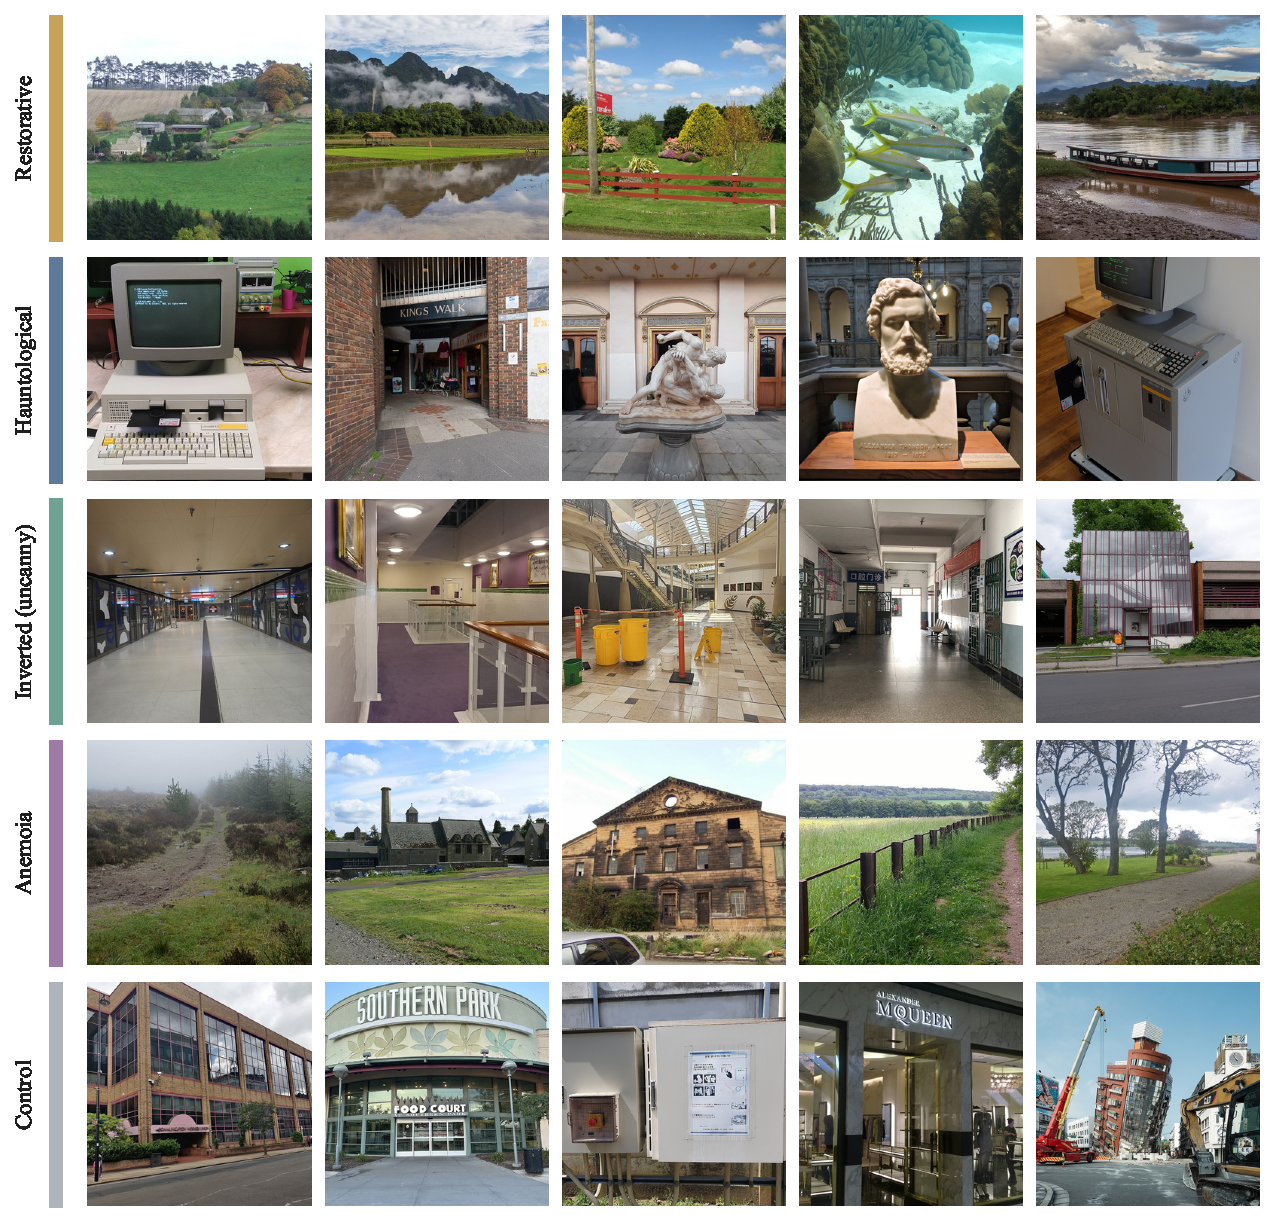
\includegraphics[width=0.92\linewidth]{figures/fig0_examples.pdf}
\caption{Representative stimuli per cluster (the five images nearest each cluster
centroid in standardized feature space; genuine exemplars). Top to bottom: restorative
(nature/water/sky, glossy optimism), hauntological (busts, CRT-era electronics: ``lost
futures''), inverted (empty corridors, malls, lots: liminal/kenopsia), anemoia (estates,
misty forests, libraries), control (the same scene types as inverted, populated).}
\label{fig:examples}
\end{figure}

Restorative (R). Warm, comfort-seeking, techno-optimist: Frutiger Aero,
Frutiger Eco, Y2K/Cybercore, cottagecore, kidcore, and the optimistic strand of
retro-futurism (Googie, atomic-age, synthwave). The past, or the past's imagined future,
recalled as good (Boym's restorative pole; \citealp{boym2001}).

Hauntological (H). Ironic, melancholic, ambivalent: vaporwave, mallsoft,
chillwave, and the decayed strand of retro-futurism (cassette futurism, dieselpunk).
Fisher's lost futures: longing inflected by the knowledge that the promised future did
not arrive.

Anemoia (A). Longing for unlived, often never-existent pasts: dark academia,
light academia, fairycore, goblincore, royaltycore, old money. Nostalgia fully detached
from autobiography.

Inverted / uncanny (I). Nostalgia stripped of comfort: liminal spaces (the
term adapted from ritual liminality, the unstable in-between phase of a rite of passage;
\citealp{turner1969}), the Backrooms, poolrooms, dreamcore, weirdcore, traumacore, analog
horror. The eerie in Fisher's sense, where something that should be present is absent, as
in a place with no people \citep{fisher2016}. This family connects nostalgia to the uncanny
proper \citep{jentsch1906, freud1919, mori2012}, whose modern accounts emphasize realism
inconsistency \citep{macdorman2016} and configural deviation from the familiar
\citep{diel2022meta, diel2022}.

Control (C). Ordinary, populated, present-day scenes: the non-nostalgic baseline
against which the others are measured, and the reference distribution for the $\phi$ coordinates.


Each image is reduced to a compact set of image-computable coordinates: three perceptual axes
and four mechanism coordinates $\phi$. The perceptual axes capture colour and gloss (the
restorative signature), structural emptiness and human absence from ADE20K segmentation
\citep{xie2021} (the eerie signature), and an expected-but-absent object score from
open-vocabulary detection \citep{minderer2023}. The four $\phi$ coordinates place each image
relative to ordinary present-day scenes: typicality (distance from the per-scene control
centroid), surprise (reconstruction error off the control manifold), realism variance, and scene
entropy. The reference for every $\phi$ is estimated on present-day controls alone, which keeps
the coordinates independent of any model rating or interpretation applied later. Full definitions,
the DINOv2/CLIP backbone, and statistical procedures appear in Supplementary Material~S1-S4.
Together the axes and $\phi$ form the affective-temporal space, and the clusters are regions
within it.

\section{Results}


The evidence arrives in three movements: a global map of how the aesthetics relate, a check that
the map survives when rebuilt from a second and unrelated record of behaviour, and a test of
whether the same structure is legible in the images themselves and to frontier vision-language
models.

The map comes first. Treating the Aesthetics Wiki as a behavioural record (Methods;
Supplement~S6), we enumerate every article that carries an aesthetic infobox and parse its
\textsc{related\_aesthetics} field, which yields a network of $1{,}115$ aesthetics joined by
$5{,}889$ human-drawn links. It forms a single connected component, so internet aesthetics are one
cultural fabric rather than a scatter of isolated scenes, and that fabric is highly structured:
Louvain community detection finds $13$ communities with modularity $Q=0.526$, against a
degree-preserving rewired null of $Q=0.007$ (Fig.~\ref{fig:ecosystem}).

Two latent axes organise that partition, and the first is affect. Scoring each aesthetic's
community-authored \textsc{key\_values} on a fixed four-dimension lexicon (unease, nostalgia,
comfort, refinement), edges that join two aesthetics of the same dominant affect outnumber a
label-permutation null by a wide margin ($537$ of $1{,}249$ such edges, against $353$ expected;
$p=0.0005$). Affect organises the graph, and it does so across the grain: the communities are
mostly subcultural (goth, punk, steampunk; cottagecore and nature; academia; futurism), with
affect running as a gradient within and between them rather than carving out communities of its
own. The second axis is time. Community median \textsc{decade\_of\_origin} climbs from the $1920$s
(modernism, art nouveau) through the $1950$s (mid-century, retro-futurism) and $1980$s (punk, goth)
to the $2010$s (the internet-native cluster), a second and orthogonal organiser.

The four-way affective-mechanism taxonomy we specify on theoretical grounds (restorative,
hauntological, anemoia, inverted) aligns with the network's unsupervised communities:
locating our $23$ seed aesthetics in the network, the normalised mutual information between their
a-priori cluster and their (label-free) community is $\mathrm{NMI}=0.50$ (permutation null
$0.27$, $p=0.002$). The alignment is partial, with restorative aesthetics in particular scattering
across several communities, and it sits well above chance, obtained with no researcher labels
entering the community detection.

\begin{sidewaysfigure}
\centering
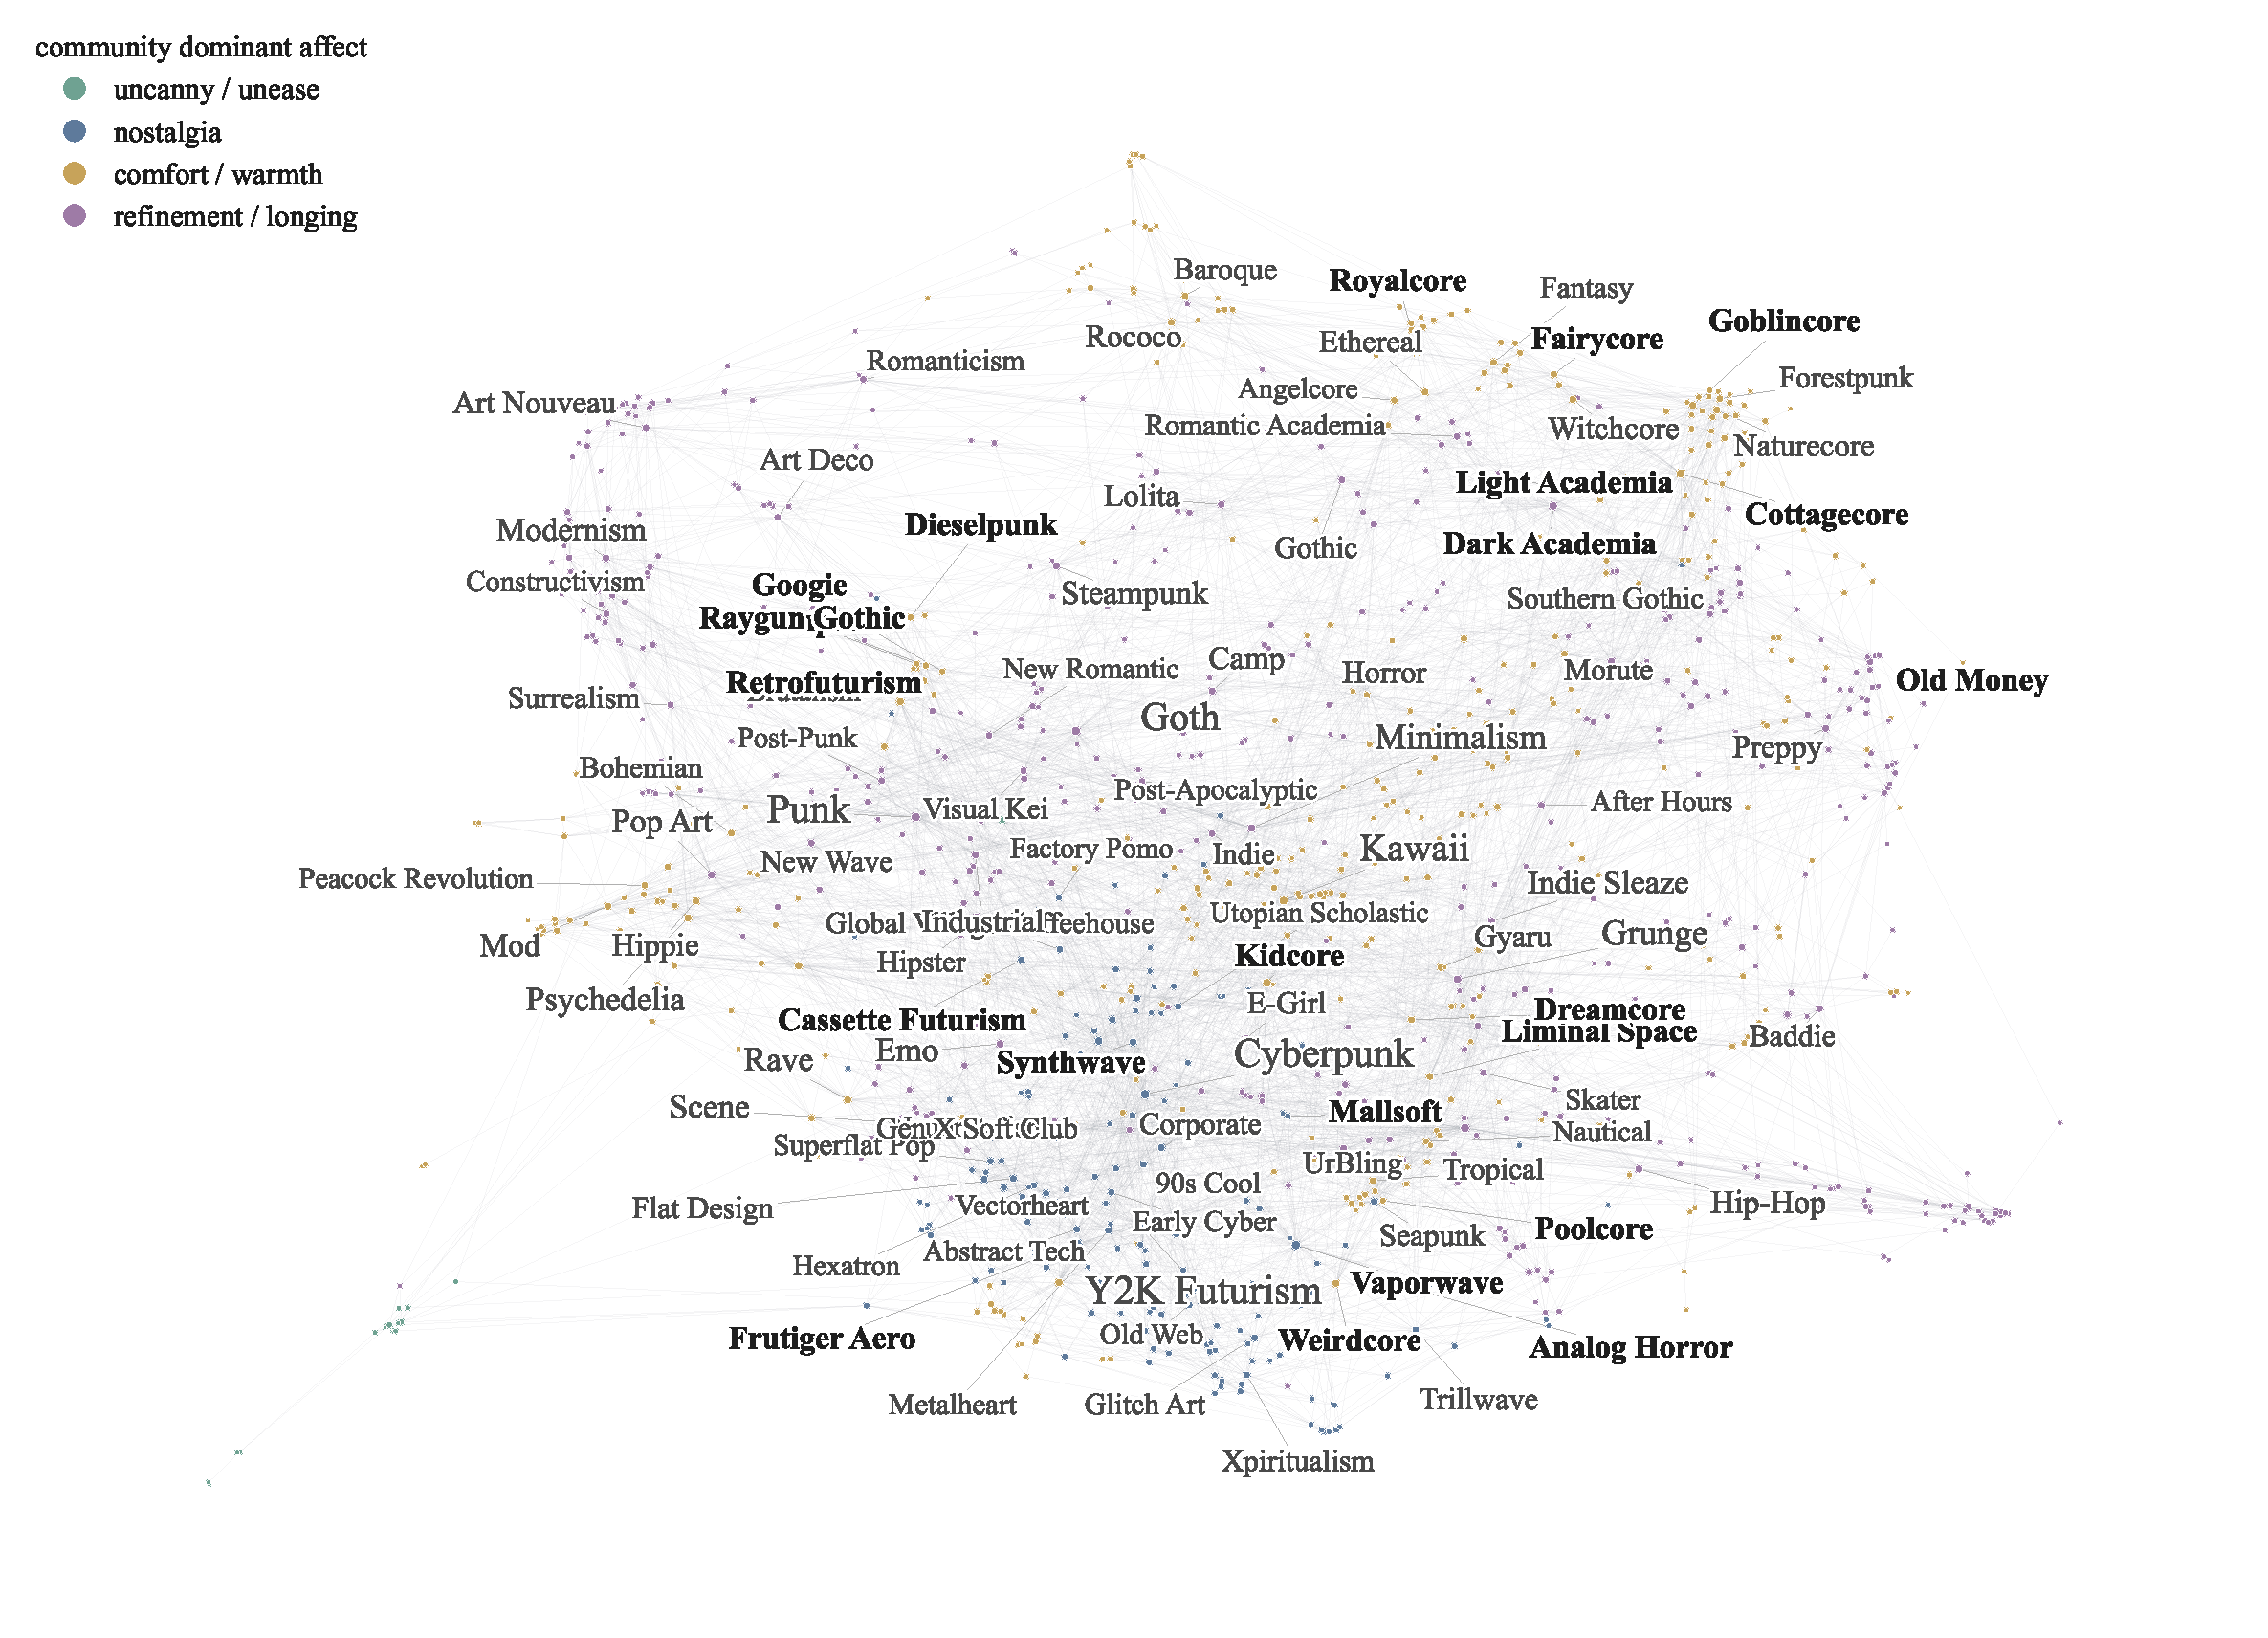
\includegraphics[width=\textheight]{figures/ecosystem_network.pdf}
\caption{The internet-aesthetics curation network. $1{,}115$ aesthetics joined by
$5{,}889$ community-authored ``related'' links, laid out by a force-directed algorithm
(ForceAtlas2). Nodes are coloured by their community's dominant community-authored affect and
sized by curatorial degree. All $1{,}115$ aesthetics are plotted; $100$ are labelled (the $26$
focal aesthetics in bold, the highest-degree hubs in grey, font scaled by degree); an interactive
explorer of the full set is released with the data. The network is strongly
modular ($13$ Louvain communities, $Q=0.53$ vs.\ a $0.01$ rewired null), and communities
separate systematically by affect ($p=0.0005$) and by era (1920s to 2010s).}
\label{fig:ecosystem}
\end{sidewaysfigure}

The map so far rests on a single behavioural trace, the editors' \textsc{related} links, so its
modularity could in principle reflect how one community writes cross-references. The second
movement rebuilds the network from unrelated behaviour: are.na user co-curation. For every harvested image we
retrieved the full set of channels users filed it into, mapped channel titles to aesthetics, and
linked two aesthetics whenever users co-filed the same image under both, a record of curation
behaviour that shares no mechanism with wiki editing. The resulting co-curation graph ($104$
aesthetics, $354$ edges) has sensible structure (top pairs: Fairycore and Fairytale,
Cassette Futurism and Futurism, Dreamcore and Weirdcore), and its
communities align with the wiki communities above chance on the $103$ shared aesthetics
($\mathrm{NMI}=0.21$ versus a label-permutation null of $0.17$, $p=0.032$). The agreement is modest
and significant: two independent traces of collective behaviour converge, which places the
community structure beyond a single editorial source.


The third movement turns from how people relate aesthetics to the images themselves, where the
modes are visible directly in content. On the openly-licensed corpus
($N=681$; Wikimedia Commons), a five-way classifier over the perceptual features separates
the modes above chance (cross-validated accuracy $0.57$; permutation $p<0.01$), and the
inverted/uncanny pole occupies a region of high structural human-absence, separating from
scene-matched populated controls within category (Cohen's $d=0.38$, 95\% CI $[0.14,0.68]$).
An independent CLIP observer reproduces the same inverted-vs-rest eerie ordering ($d=0.72$,
95\% CI $[0.47,0.99]$), foreshadowing the frontier-model analysis below. Feature definitions,
the classifier decomposition, the per-scene cells, and the CLIP probes are given in
Supplementary~Sec.~\ref{sup:imgstruct}.


CLIP encodes human associations only indirectly, so we tested the taxonomy against two
sources of explicit collective human labelling, harvested from the community-run Aesthetics
Wiki and the curation platform are.na (Supplement~S6). Both records are observational, and we state
their limits below; each provides a human criterion external to our features and our corpus.

The first source is community-authored affect: each Aesthetics-Wiki page carries a structured
\textsc{key\_values} field naming the aesthetic's affective content, and 21 of our 26 named aesthetics
populate it. Scoring these against a pre-specified four-dimension affect lexicon (unease,
nostalgia, comfort, refinement) recovers the predicted structure. The uncanny (inverted) cluster
dominates unease ($d=2.66$ versus all other clusters pooled); restorative aesthetics are
described overwhelmingly in terms of comfort, and anemoia almost entirely in terms of
refinement (intellectualism, elegance, tradition). Nostalgia is named across
restorative (50\% of aesthetics), hauntological (75\%), and inverted (80\%) aesthetics, direct
community evidence that nostalgia is a shared substrate across modes, the paper's central claim.
Anemoia is the informative exception: the community labels it with refinement terms and uses the
word nostalgia for none of its aesthetics (0\%), consistent with anemoia being a longing for an
unlived past that feels distinct from remembered nostalgia.

The second source is a crowd-drawn similarity graph: each page also lists \textsc{related
aesthetics}, yielding a crowd-authored similarity network. Restricting to the 73 edges
whose endpoints both fall in our taxonomy, the fraction joining two aesthetics of the
same affective-mechanism cluster is $0.49$, against a label-permutation null of
$0.23$ ($p=0.0006$, 5000 permutations). Independent human judgements of which aesthetics
``go together'' thus recover the R/H/I/A grouping far above chance, and unlike the lexicon
analysis this test uses no researcher-defined word list, so it avoids circularity.

The two preceding tests are category-level; the strongest
test is whether our image features predict, at the image level, the aesthetic that humans assigned each
image to. We harvested $\approx$1{,}900 are.na images whose channel placement is a crowd
membership label, extracted the same feature set, and asked a random forest to predict the label
under channel-grouped cross-validation, holding all images from one channel out together so
the model cannot exploit a single curator's house style or near-duplicates (Supplement~S6).
Structural features predict the four-way mechanism cluster at $0.42$ (majority baseline $0.29$;
permutation null $0.28$; $z=12.4$, $p<0.005$, 200 shuffles) and the 20-way specific aesthetic at
$0.13$ (chance $0.07$; $z=10.2$, $p<0.005$): well above chance, and modest in absolute terms, as
the heavy cluster overlap predicts. Two facts echo the main analysis: dropping the $\phi$
coordinates barely changes accuracy ($0.41$), so the perceptual axes carry the signal; and
anemoia is again the worst-recovered class, dispersing into the three other modes, which
marks it as the least distinct visual mode. The confusions track genuine visual kinship
(Frutiger Aero with Y2K, vaporwave with cassette futurism, dark academia with old money).

The generalizable signal is in collective association. Training the classifier on one
corpus and predicting the other, disjoint corpus (are.na, human-curated; Wikimedia,
keyword-sourced) transfers above chance (are.na$\to$Wikimedia accuracy $0.38$ vs.\ $0.35$ majority,
$z=3.2$; reverse $0.32$ vs.\ $0.30$, $z=2.5$). The structure that generalizes across independent
records therefore resides chiefly in how people collectively curate and relate aesthetics,
consistent with the network and co-curation results above, and less in low-level image statistics
specific to any one source.

Three tests across two unrelated sources of collective human labelling (category affect terms, a
crowd similarity graph, and image-level membership) corroborate a taxonomy derived on theoretical
grounds, with no rating study run.


The collective-human structure invites a machine-cognition question that needs no rating study:
whether frontier vision-language models (VLMs), trained on web-scale human image-text data and
never on this taxonomy, perceive the same affective structure, and where their reading fails. We
assembled a three-model panel (Gemini 2.5 Flash, GPT-4o, and Claude Sonnet 4.6; API identifiers
\texttt{gemini-2.5-flash}, \texttt{gpt-4o}, \texttt{claude-sonnet-4-6}) and had each rate
every are.na image on calibrated 1-5 affect scales (eerie, nostalgic, abandoned, dreamlike,
valence, arousal) and force-choose one mechanism mode. We used rubric anchors and a ``reserve~5
for unambiguous cases'' instruction because VLM affect ratings are known to inflate, and a
three-judge consensus is the recommended mitigation \citep{aicabench2026}.

The judges agree, and they track human curation. Inter-model agreement is high
(pairwise Pearson on the $1{,}115$ images rated by all three: eerie $r=0.76$, dreamlike $0.77$,
nostalgic $0.74$, valence $0.72$, arousal $0.70$; mode agreement $0.70$), so the consensus is a
reliable, shared measurement. The six consensus affect axes predict the aesthetic that
humans assigned each image to: under channel-grouped cross-validation, a random forest on the
affect axes of the two fully-covered judges reaches $0.45$ accuracy across the four modes
(majority $0.29$; permutation null $0.26\pm0.01$; $z=18.1$, $n=1{,}727$). Adding the third judge on
the images it covers leaves this unchanged (two-judge $0.60$ vs.\ three-judge $0.62$ on that
subset, where the majority baseline is itself $0.48$), so the prediction is robust to model
composition. It matches the $0.42$ achieved by our hand-built structural features, at a higher
effect size: a handful of numbers a frontier model emits about an image's feeling recover
human curatorial categories as well as a 29-dimensional perceptual description.

The models' categorical
judgements expose a systematic, directional failure (Fig.~\ref{fig:vlmbreak}). Against the human modes,
consensus mode-match is near-ceiling for the inverted/uncanny class (recall $0.86$) and
much lower for restorative ($0.35$) and anemoia ($0.31$). The misclassifications are
systematic: warmth and longing leak specifically into ``inverted'' (restorative$\to$inverted
$0.31$; anemoia$\to$inverted $0.35$), and all three models independently label the techno-optimist
flagship Frutiger Aero as ``hauntological.'' Frontier VLMs over-attribute unease,
reading the eerie into images humans experience as comforting or wistful. The effect is
affect-inflation localized to a single, culturally loaded axis, the uncanny, and it is the paper's
clearest machine-cognition result: for these models the difficult operation is to withhold
the uncanny.

\begin{figure}[t]
\centering
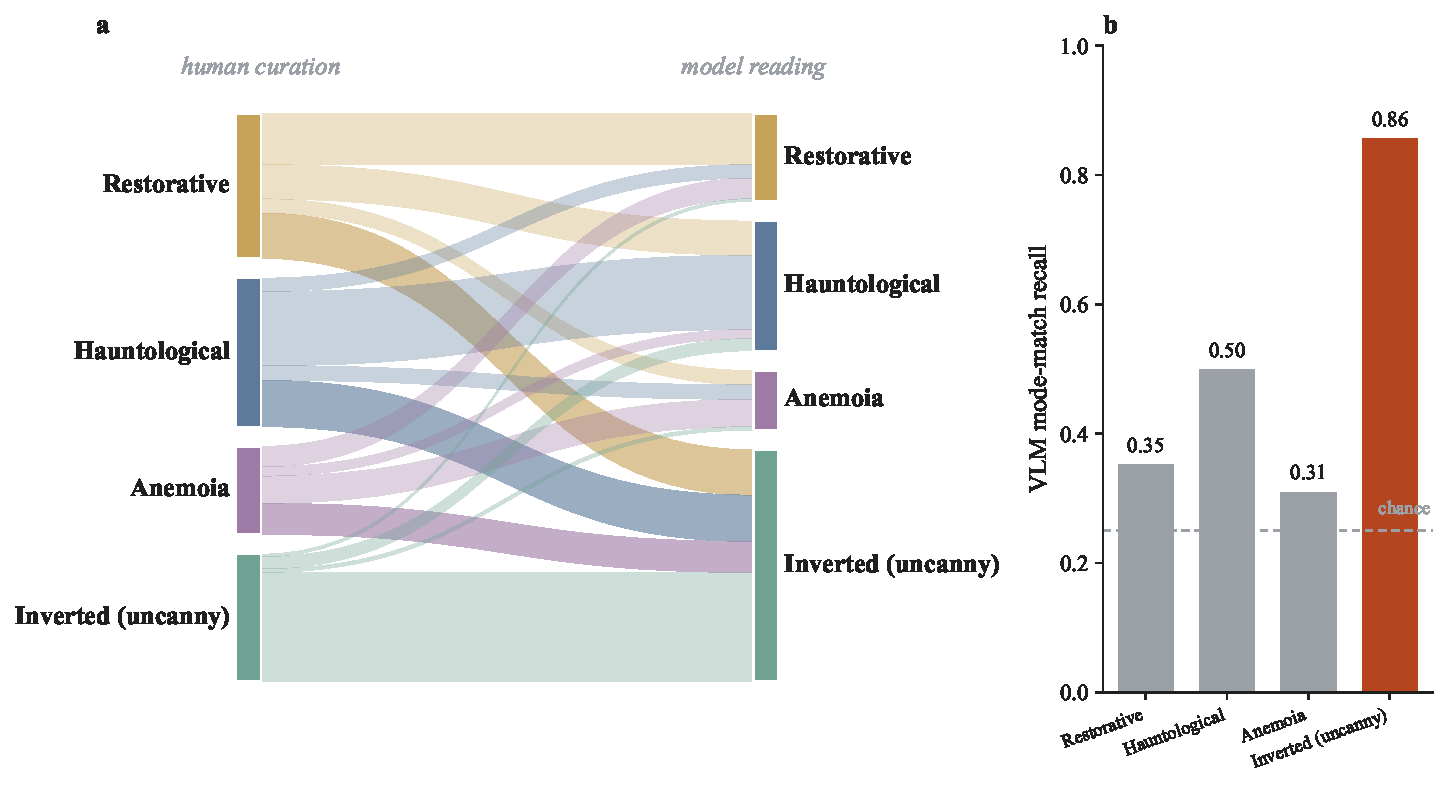
\includegraphics[width=\textwidth]{figures/vlm_flow.pdf}
\caption{The asymmetric leak into the uncanny. Three-model consensus (Gemini 2.5 Flash, GPT-4o,
Claude Sonnet 4.6) over $1{,}885$ are.na images. (a) Flow from human-assigned mode to VLM consensus mode:
each warm genre sends about a third of its images into ``inverted'' (restorative $0.31$,
hauntological $0.31$, anemoia $0.35$), while ``inverted'' retains $0.86$ of its own and leaks little
back, so unease acts as a sink. (b) Per-mode mode-match recall: near-ceiling for the uncanny and
near chance for the warm genres. The full confusion matrix appears in the Supplement
(Fig.~\ref{fig:confusionheat}).}
\label{fig:vlmbreak}
\end{figure}

A human-anchored boundary test separates two possibilities: the over-attribution could be a generic VLM
negativity bias, or something specific to internet aesthetics. We tested it against human
ground truth on OASIS \citep{oasis2017}, $\sim$890 images with normative valence/arousal ratings
($N\!\approx\!100$ each), rated by all three models. Every model tracks the human valence norm
closely (Pearson $r=0.85$, $0.84$, $0.87$ for Gemini, GPT-4o, Claude), with a small negativity
offset ($-0.02$ to $-0.07$ on a $0$ to $1$ scale), and all three reserve low \textsc{eerie} for
human-positive images (mean $1.2$ to $1.3$ of $5$). On ordinary affective images the models are
well-calibrated against people. The over-attribution is therefore domain-specific to
internet aesthetics: the failure is localised to the ambiguous, culturally-constructed visual
genres, which makes it a finding about cultural perception (Fig.~\ref{fig:oasis}).

\begin{figure}[t]
\centering
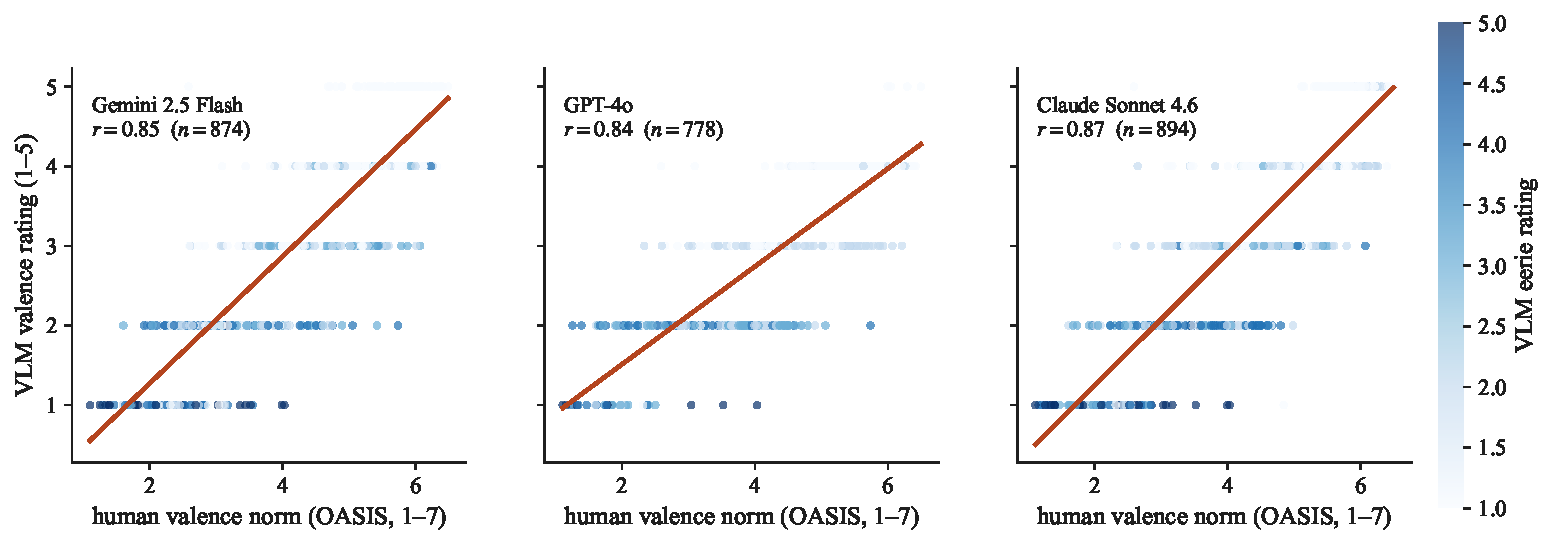
\includegraphics[width=\textwidth]{figures/oasis_calibration.pdf}
\caption{The bias is bounded: models are calibrated on standard affective images.
VLM valence vs.\ human-norm valence on OASIS, per model; points coloured by the model's
\textsc{eerie} rating. All three track human valence ($r=0.85/0.84/0.87$) and concentrate high
eerie (dark) at low human valence, reserving unease for genuinely negative scenes. On standard
affective images the models stay calibrated; the over-attribution appears on internet aesthetics.}
\label{fig:oasis}
\end{figure}


We traced the cause by dissecting the are.na images humans filed as restorative or anemoia while a
model rated them eerie ($\geq3$), with one correlational and two causal tests.

Within these naturally-warm images, a correlational test shows the
model's \textsc{eerie} rating is barely predicted by low-level image statistics: brightness, saturation,
colourfulness, edge density, gloss, blur (Laplacian variance) and resolution together explain
almost none of the variance (standardised multiple regression $R^2=0.04$; the only sizeable term
is structural emptiness, $\beta=0.22$). Eeriness stands independent of degradation and palette.

A first intervention edits the image: we naturalised 120 such images by
denoising, upscaling and sharpening (quality), and by restoring brightness, contrast and
saturation (tone), then re-rated them. Every manipulation left eeriness at or above its original
level (full naturalization: Gemini $\Delta=+0.08$, 95\% CI $[-0.04,+0.21]$ and GPT-4o
$+0.06\,[-0.03,+0.15]$, both n.s.; Claude $+0.12\,[+0.03,+0.22]$). Making an internet-aesthetic
image look like a clean photograph leaves the attributed unease in place, so its cause lies
beyond the processed appearance.

A second intervention changes only the question, holding the image fixed. Reframing the rating to ``the scene depicted, rather than its visual
style'' lowered eeriness in every model, and an explicit debias (``stylisation, such as filters,
grain, low resolution, text, and retro grading, is not evidence of threat'') lowered it further:
$\Delta=-0.72$ (95\% CI $[-0.87,-0.58]$) for Gemini, $-0.24\,[-0.33,-0.16]$ for GPT-4o, and
$-0.37\,[-0.50,-0.23]$ for Claude, all reliably below zero. The pixels were fixed, and a
one-sentence reframe moved the rating toward calibration in all three (Fig.~\ref{fig:mechanism}).

\begin{figure}[t]
\centering
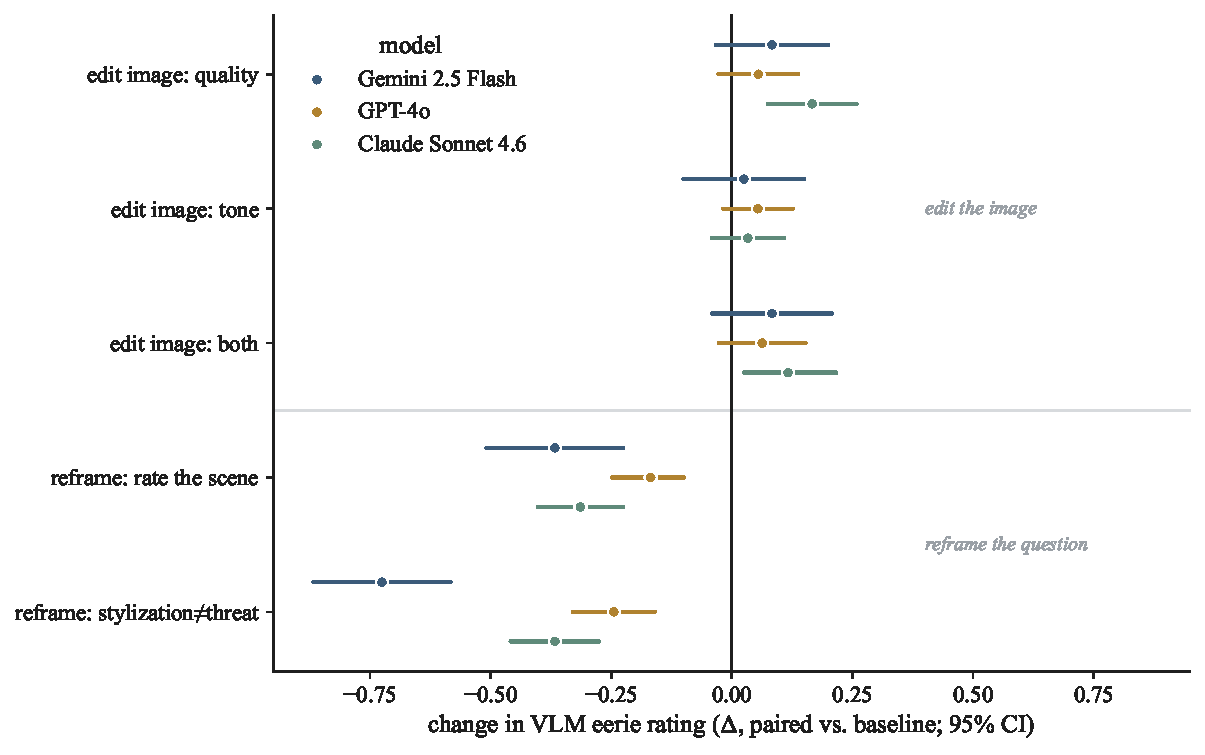
\includegraphics[width=0.82\textwidth]{figures/mechanism_forest.pdf}
\caption{The over-attribution operates at the level of interpretation. Paired change in
VLM \textsc{eerie} for each manipulation, per model (95\% CI). Editing the image (denoise,
upscale, recolour) never lowers eeriness (intervals at or above zero) in any model; reframing the
question (rate the scene; treat stylisation as benign) lowers it (intervals left of zero).
The cause lies in interpretation.}
\label{fig:mechanism}
\end{figure}

The convergent picture is that frontier VLMs treat stylisation
itself, the visual signature of a curated internet aesthetic, as evidence of wrongness, and they
do so at the level of interpretation: the bias is invisible in the image statistics, it
survives editing of the image, and it is largely correctable by reframing the task. This is the
visual, affective counterpart of exaggerated safety in language models, where benign inputs
that merely look risky are treated as unsafe \citep{rottger2024}, and of the broader tendency of
frontier models to amplify, and sometimes invent, evaluative biases \citep{cheung2025,
gallegos2024}; here the surface cue is a genre's post-processing in place of a keyword. It also
yields a practical fix: affective-computing pipelines that elicit scene-level affect, in place of
style-level affect, substantially debias VLM unease.

\begin{figure}[t]
\centering
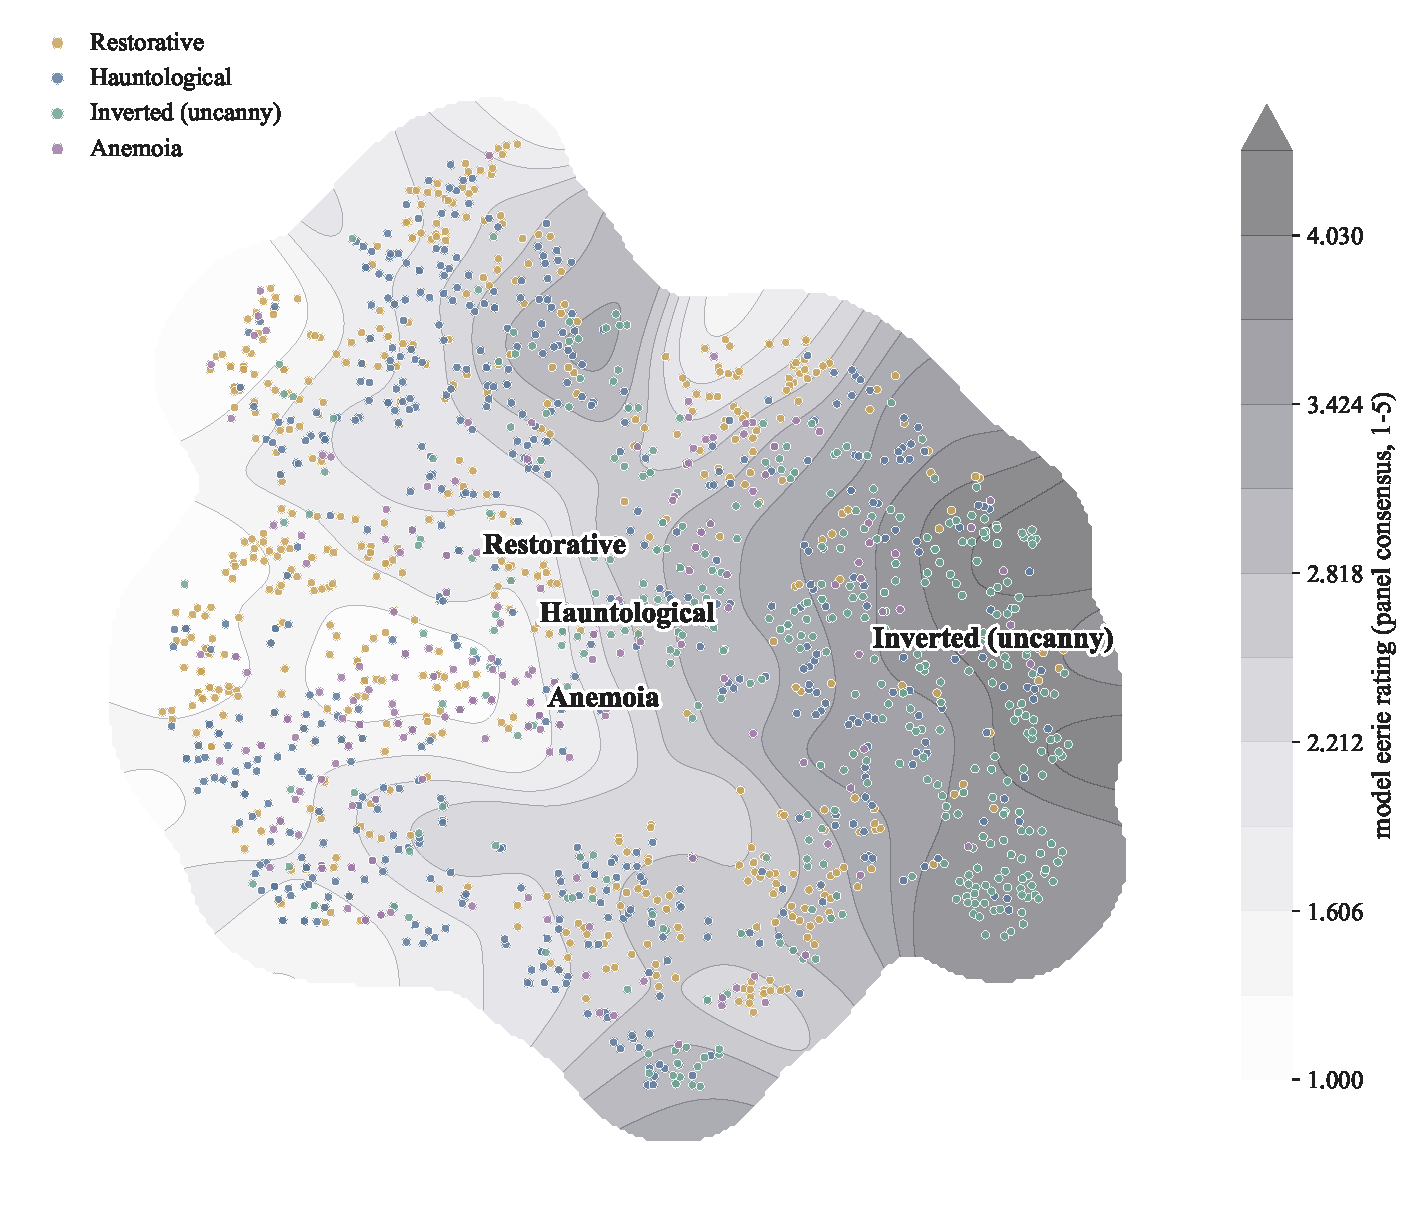
\includegraphics[width=0.84\textwidth]{figures/manifold_uncanny.pdf}
\caption{The panel's affective landscape. Each are.na image is embedded (t-SNE) by the panel's
non-eerie affect ratings (valence, arousal, nostalgic, abandoned, dreamlike) and coloured by its
human-assigned mode; the eerie rating, withheld from the embedding, is overlaid as a smoothed
shadow field. Eerie rises toward the uncanny pole, and warm-labelled images carry a modest eerie
elevation throughout. The map is a descriptive view of the model's affect space; the causal
evidence for the over-attribution is Figs.~\ref{fig:vlmbreak}--\ref{fig:mechanism}.}
\label{fig:atlas}
\end{figure}

\section{Discussion}

Three independent windows on internet visual culture (how an online community cross-references
aesthetics, how users co-curate images, and how frontier vision-language models perceive those
images) converge on a common affective architecture, and that convergence is this paper's
throughline. The architecture stays consistent across independent records: a network built from
editors' cross-references is strongly modular and organized by latent affect and historical era;
a second record of user co-curation aligns with the same communities above chance
($\mathrm{NMI}=0.21$ vs.\ a $0.17$ null, $p=0.032$); and those unsupervised communities align with the four-mode taxonomy
($\mathrm{NMI}=0.50$). The signal is carried chiefly by collective association, how people
group and curate aesthetics, and only in part by low-level pixels, which transfer across sources
weakly ($z\!\approx\!3$). What the analysis recovers is the culture's own affective organization,
read from behaviour.

The architecture's most striking property is that systems never trained on it perceive it: a
frontier panel predicts human curatorial categories from affect ratings alone, as accurately as a
29-dimensional perceptual description ($z=18$). That legibility is biased in a
specific direction: the models reach near-ceiling on the uncanny while reading warmth and longing
as eerie, over-attributing unease along the most culturally loaded axis. Three diagnostics localize
the cause: the over-attribution is absent from image statistics, it is unchanged by naturalizing
the image, and it falls sharply when the rating question is reframed, so it operates at the level
of interpretation, with the models treating stylization itself as evidence of wrongness. Across the
panel's affect space the eerie field forms a shadow that spreads from the uncanny pole into the warm
territories, the same over-attribution seen image by image (Fig.~\ref{fig:atlas}). It is
also bounded: on standardized affective images the models match human valence norms ($r=0.84$ to
$0.87$) and reserve eeriness for genuinely negative scenes. The phenomenon, its boundary, and its
causal mechanism hold across Gemini, GPT-4o and Claude, so the bias is a property of current
frontier VLMs broadly. It extends the exaggerated-safety phenomenon documented for language
inputs \citep{rottger2024} into culturally coded visual affect: a directional, diagnosable,
bounded, and correctable bias, with direct consequences for affective-computing systems that
elicit style-level affect in place of scene-level affect.

These results also bear on nostalgia itself, since the aesthetics of the feed externalize at least
four operations on the past, restoring it, mourning its lost futures, inventing one never lived, and
inverting it into unease, and both the human records and the models place the uncanny within
nostalgia, as its inversion. Anemoia is the least pictorially distinct of the four, dispersing
across communities and proving the hardest mode for both features and models, consistent with its
coherence being conceptual, a shared relation to an unlived past, as much as visual.

\section{Limitations}

Three boundaries frame the scope of these results. First, the evidence is observational: the
affective criteria are existing human records (community descriptions, are.na curation) and
standardized norms in place of first-party ratings, which buys naturalism and scale while ceding
experimental control over what each criterion isolates. Second, the are.na curators and
wiki editors are a design-literate online population, so the recovered ``human'' structure
reflects how that community organizes visual culture. Third, the openly-licensed image corpus
indexes the subject matter of some aesthetics more than their post-processing, which is why the
central image-level and model analyses use the are.na corpus, curated by people as instances of
each aesthetic. The over-attribution, the OASIS boundary, and the causal mechanism are each
established across all three frontier models (Gemini, GPT-4o, Claude); we cannot say whether the
effect extends to closed reasoning models or to future architectures.

\section{Conclusion}

Internet visual culture has a measurable affective architecture, and that architecture is
legible to the machines now trained on the same culture. Reading two independent records of
collective curation, we recover a modular network of aesthetics organized by affect and era, and
a four-mode taxonomy that its unsupervised communities align with. A frontier panel recovers the
same structure from images alone, predicting human curatorial categories from affect, and it
over-attributes unease to culturally constructed warm and wistful genres. We trace that bias to
interpretation: it is absent from the pixels, it survives editing of them, it is bounded (the
models match human affect norms on standardized images), and it falls substantially when the
rating task is reframed. The result is a diagnosable, bounded, and correctable failure mode of
frontier affective perception, with a practical fix for systems that read affect from culturally
stylized imagery.

Data and code availability. We release, as an open archive on Zenodo
(\href{https://doi.org/10.5281/zenodo.20698074}{DOI: 10.5281/zenodo.20698074}): the aesthetics catalogue and ecosystem network
($1{,}115$ aesthetics with affect, era, and related-aesthetic links), with a self-contained
interactive HTML explorer of the full network (pan, zoom, search); the are.na human-label
and co-curation records; the openly-licensed $681$-image corpus with per-image attribution and
its feature table; the three-model frontier affect ratings and the OASIS benchmarking and
mechanistic-intervention outputs; and all harvest and analysis code. The compilation is CC-BY-4.0;
licensed images retain their individual CC / public-domain licences. are.na images are
copyright-held and were used for feature extraction only and are not redistributed.

\begin{thebibliography}{99}
% - nostalgia -
\bibitem[Boym(2001)]{boym2001} Boym, S. (2001). \emph{The Future of Nostalgia}. Basic
Books.
\bibitem[She et al.(2026)]{aicabench2026} She, D., Yao, X., Chen, L., Yu, J., Gao, Y., \&
Jin, Z. (2026). AICA-Bench: holistically examining the capabilities of vision-language models in
affective image content analysis. \emph{Preprint}, arXiv:2604.05900.
\bibitem[Kurdi et al.(2017)]{oasis2017} Kurdi, B., Lozano, S., \& Banaji, M. R. (2017).
Introducing the Open Affective Standardized Image Set (OASIS). \emph{Behavior Research
Methods}, 49(2), 457-470.
\bibitem[Wildschut et al.(2006)]{wildschut2006} Wildschut, T., Sedikides, C., Arndt, J.,
\& Routledge, C. (2006). Nostalgia: content, triggers, functions. \emph{Journal of
Personality and Social Psychology}, 91(5), 975-993.
\bibitem[Routledge et al.(2011)]{routledge2011} Routledge, C., Arndt, J., Wildschut, T.,
et al. (2011). The past makes the present meaningful: nostalgia as an existential
resource. \emph{Journal of Personality and Social Psychology}, 101(3), 638-652.
\bibitem[Sedikides \& Wildschut(2018)]{sedikides2018} Sedikides, C., \& Wildschut, T.
(2018). Finding meaning in nostalgia. \emph{Review of General Psychology}, 22(1), 48-61.
\bibitem[Batcho(1995)]{batcho1995} Batcho, K. I. (1995). Nostalgia: a psychological
perspective. \emph{Perceptual and Motor Skills}, 80(1), 131-143.
% - memory / anemoia -
\bibitem[De Brigard(2014)]{debrigard2014} De Brigard, F. (2014). Is memory for
remembering? Recollection as a form of episodic hypothetical thinking. \emph{Synthese},
191(2), 155-185.
% - hauntology / liminality -
\bibitem[Fisher(2014)]{fisher2014} Fisher, M. (2014). \emph{Ghosts of My Life:
Writings on Depression, Hauntology and Lost Futures}. Zero Books.
\bibitem[Fisher(2016)]{fisher2016} Fisher, M. (2016). \emph{The Weird and the Eerie}.
Repeater Books.
\bibitem[Turner(1969)]{turner1969} Turner, V. (1969). \emph{The Ritual Process:
Structure and Anti-Structure}. Aldine.
% - the uncanny -
\bibitem[Jentsch(1906/1997)]{jentsch1906} Jentsch, E. (1906/1997). On the psychology of
the uncanny. \emph{Angelaki}, 2(1), 7-16.
\bibitem[Freud(1919/1955)]{freud1919} Freud, S. (1919/1955). The uncanny (Das
Unheimliche). In \emph{The Standard Edition of the Complete Psychological Works of
Sigmund Freud}, Vol.\ 17 (pp.\ 217-256). Hogarth Press.
\bibitem[Mori et al.(2012)]{mori2012} Mori, M., MacDorman, K. F., \& Kageki, N. (2012).
The uncanny valley (1970). \emph{IEEE Robotics \& Automation Magazine}, 19(2), 98-100.
\bibitem[MacDorman \& Chattopadhyay(2016)]{macdorman2016} MacDorman, K. F., \&
Chattopadhyay, D. (2016). Reducing consistency in human realism increases the uncanny
valley effect; increasing category uncertainty does not. \emph{Cognition}, 146, 190-205.
\bibitem[Diel et al.(2022)]{diel2022meta} Diel, A., Weigelt, S., \& MacDorman, K. F.
(2022). A meta-analysis of the uncanny valley's independent and dependent variables.
\emph{ACM Transactions on Human-Robot Interaction}, 11(1), 1-33.
\bibitem[Diel \& Lewis(2022)]{diel2022} Diel, A., \& Lewis, M. (2022). Structural deviations
drive an uncanny valley of physical places. \emph{Journal of Environmental Psychology}, 82, 101844.
% - predictive processing -
\bibitem[Friston(2010)]{friston2010} Friston, K. (2010). The free-energy principle: a
unified brain theory? \emph{Nature Reviews Neuroscience}, 11(2), 127-138.
\bibitem[Clark(2013)]{clark2013} Clark, A. (2013). Whatever next? Predictive brains,
situated agents, and the future of cognitive science. \emph{Behavioral and Brain
Sciences}, 36(3), 181-204.
% - computational backbone -
\bibitem[Hasler \& S\"usstrunk(2003)]{hasler2003} Hasler, D., \& S\"usstrunk, S. (2003).
Measuring colourfulness in natural images. \emph{Proc.\ SPIE Human Vision and Electronic
Imaging}, 5007, 87-95.
\bibitem[Radford et al.(2021)]{radford2021} Radford, A., et al. (2021). Learning
transferable visual models from natural language supervision (CLIP). \emph{ICML}.
\bibitem[Xie et al.(2021)]{xie2021} Xie, E., et al. (2021). SegFormer: simple and
efficient design for semantic segmentation with transformers. \emph{NeurIPS}.
\bibitem[Minderer et al.(2023)]{minderer2023} Minderer, M., Gritsenko, A., \& Houlsby, N.
(2023). Scaling open-vocabulary object detection (OWLv2). \emph{NeurIPS}.
\bibitem[Oquab et al.(2024)]{oquab2024} Oquab, M., et al. (2024). DINOv2: learning robust
visual features without supervision. \emph{Transactions on Machine Learning Research}.
% - visual emotion / aesthetics / memorability datasets -
\bibitem[Murray et al.(2012)]{murray2012} Murray, N., Marchesotti, L., \& Perronnin, F.
(2012). AVA: a large-scale database for aesthetic visual analysis. \emph{CVPR}.
\bibitem[Khosla et al.(2015)]{khosla2015} Khosla, A., Raju, A. S., Torralba, A., \& Oliva,
A. (2015). Understanding and predicting image memorability at a large scale (LaMem).
\emph{ICCV}.
\bibitem[Achlioptas et al.(2021)]{achlioptas2021} Achlioptas, P., Ovsjanikov, M., Haydarov,
K., Elhoseiny, M., \& Guibas, L. (2021). ArtEmis: affective language for visual art.
\emph{CVPR}.
\bibitem[Yang et al.(2023)]{yang2023} Yang, J., et al. (2023). EmoSet: a large-scale visual
emotion dataset with rich attributes. \emph{ICCV}.
\bibitem[Mertens et al.(2024)]{mertens2024} Mertens, L., et al. (2024). FindingEmo: an image
dataset for emotion recognition in the wild. \emph{Preprint}, arXiv:2402.01355.
% - VLM / LLM affective evaluation and bias -
\bibitem[Lian et al.(2023)]{lian2023} Lian, Z., et al. (2023). GPT-4V with emotion: a
zero-shot benchmark for generalized emotion recognition. \emph{Preprint}, arXiv:2312.04293.
\bibitem[Yu et al.(2026)]{vulca2026} Yu, H., Ruiz-Dolz, R., Yang, D., He, H., Zhang, F., \&
Yi, Q. (2026). VULCA-Bench: a multicultural vision-language benchmark for evaluating cultural
understanding. \emph{Preprint}, arXiv:2601.07986.
\bibitem[R\"ottger et al.(2024)]{rottger2024} R\"ottger, P., Kirk, H. R., Vidgen, B., et al.
(2024). XSTest: a test suite for identifying exaggerated safety behaviours in large language
models. \emph{NAACL}; arXiv:2308.01263.
\bibitem[Gallegos et al.(2024)]{gallegos2024} Gallegos, I. O., et al. (2024). Bias and
fairness in large language models: a survey. \emph{Computational Linguistics}, 50(3),
1097-1179.
\bibitem[Cheung et al.(2025)]{cheung2025} Cheung, V., et al. (2025). Large language models
show amplified cognitive biases in moral decision-making. \emph{PNAS},
doi:10.1073/pnas.2412015122.
\end{thebibliography}

\clearpage
\appendix
\renewcommand{\thesection}{S\arabic{section}}
\renewcommand{\thesubsection}{S\arabic{section}.\arabic{subsection}}
\renewcommand{\thetable}{S\arabic{table}}
\renewcommand{\thefigure}{S\arabic{figure}}
\renewcommand{\theequation}{S\arabic{equation}}
\setcounter{section}{0}\setcounter{table}{0}\setcounter{figure}{0}\setcounter{equation}{0}

\begin{center}\Large Supplementary Material\end{center}
\noindent The main text reports what each quantity measures; this supplement gives the
formal definitions, the model backbone and implementation, the statistical procedures, and
the computational-observer probes, so the pipeline is fully specified and reproducible.

\section{Perceptual feature definitions}

Colour and gloss: on an image in linear RGB we compute a CIELAB $k$-means palette,
saturation-weighted circular hue statistics, and the Hasler-S\"usstrunk colourfulness
\begin{equation}
\mathcal{C}=\sqrt{\sigma_{rg}^2+\sigma_{yb}^2}+0.3\sqrt{\mu_{rg}^2+\mu_{yb}^2},
\qquad rg=R-G,\;\; yb=\tfrac12(R+G)-B .
\end{equation}
The gloss index is $g=\rho_{\text{smooth}}/(\rho_{\text{edge}}+\varepsilon)$, where
$\rho_{\text{smooth}}$ is the fraction of pixels with a gentle, non-flat, non-edge
luminance gradient and $\rho_{\text{edge}}$ is the Canny edge fraction.

Structural emptiness: with structural-surface, occupant, and person area
fractions $f_{\text{struct}},f_{\text{occ}},f_{\text{person}}$ from ADE20K segmentation,
\begin{align}
\textsc{emptiness} &= f_{\text{struct}}\,\bigl(1-\min(1,\,3 f_{\text{occ}})\bigr),\\
\textsc{human\_absence} &= f_{\text{struct}}\,\bigl(1-\min(1,\,50 f_{\text{person}})\bigr).
\end{align}
The factor $50$ makes \textsc{human\_absence} collapse as soon as any person area appears,
isolating absence as distinct from bareness. We also compute a vanishing-structure measure
(longest uninterrupted structural run) and region-count / size-Gini measures.

Object expectation: with an open-vocabulary detector and a per-scene object prior
$p(o\mid s)$,
\begin{equation}
\textsc{exp\_absent}(s)=\frac{1}{Z}\sum_{o} p(o\mid s)\,\bigl(1-d(o)\bigr),
\qquad Z=\sum_o p(o\mid s),
\end{equation}
with $d(o)\in[0,1]$ the detector's maximum confidence for object $o$.

\section{Mechanism coordinates \texorpdfstring{$\phi$}{phi}}

Let $z$ be the DINOv2 \texttt{[CLS]} embedding. The reference distribution is estimated
only on present-day control images, grouped by scene category $c$ (the firewall).
\begin{align}
\phi_{\text{typ}}(z,c) &= -\,(z-\mu_c)^{\!\top}\,\Sigma_c^{-1}\,(z-\mu_c)
   && \text{(negative squared Mahalanobis; $\Sigma_c^{-1}$ Ledoit-Wolf shrinkage)}\\
\phi_{\text{surp}}(z) &= s(z) - \hat\beta^{\!\top} c_{\text{lo}}
   && \text{$s(z)=\lVert z-(\mu+WW^{\!\top}(z-\mu))\rVert^2$, $W$ a control-fit PCA basis}\\
\phi_{\text{real}} &= \operatorname{Var}_t\, r_t,\;\; r_t=P(\text{real photo}\mid\text{tile }t)
   && \text{(CLIP, $4\times4$ tiles)}\\
\phi_{\text{ent}}(z) &= -\textstyle\sum_k p_k\log p_k
   && \text{($p=\mathrm{softmax}$ of a control-trained scene classifier).}
\end{align}
In $\phi_{\text{surp}}$ the raw reconstruction error $s(z)$ is residualized on low-level
complexity covariates $c_{\text{lo}}$ (JPEG compressibility, edge density, radial
spatial-frequency slope) by a regression $\hat\beta$ fit on controls only, so the
coordinate reflects semantic surprise with textural surprise regressed out. $\phi_{\text{surp}}$ is a
pragmatic stand-in for a trained generative model's reconstruction NLL.

\section{Implementation}

SegFormer-B4 (ADE20K) for segmentation, OWLv2-base-ensemble for open-vocabulary detection,
DINOv2-base for embeddings, and CLIP ViT-B/32 for realism variance and the
computational-observer probes (S5). All models load lazily. The pipeline runs on an NVIDIA
RTX 5070 Ti (Blackwell, sm\_120), which requires a CUDA-12.8 PyTorch build (the default
wheel fails on this architecture); a full $681$-image run completes in $\approx 11$ minutes.

\section{Statistical procedures}

Cluster separability used a five-way classifier (random forest, 400 trees; and multinomial
logistic) under stratified 5-fold cross-validation, with a permutation baseline of 200
label shuffles. The firewall decomposition re-ran the random forest on the 26 non-$\phi$
features (13 colour, 10 segmentation, 3 object; \textsc{exp\_absent} excluded as
scene-tagged only) and on the three all-image $\phi$ features. Scene-matched effects are
Cohen's $d$ computed within scene category, with bootstrap 95\% CIs (2000-3000
resamples) per cell and for the sample-weighted aggregate. $\phi_{\text{typ}}$ is reported
as a percentile of the per-scene control Mahalanobis distribution in place of the raw value,
which inflates for off-distribution points in high dimensions under shrinkage.

\section{Computational-observer probes (CLIP)}

For each affective axis (eerie, nostalgic, abandoned, dreamlike) we built a positive and a
negative pole from five paraphrase prompts each, embedded with CLIP's text encoder, and
took each pole as the mean unit text embedding (prompt ensembling). For an image embedding
$v$ the score is $P(\text{positive pole})=\sigma\bigl(\tau(v\!\cdot\!t_+ - v\!\cdot\!t_-)\bigr)$
with $\tau$ the CLIP logit scale. Example eerie prompts: positive, ``an eerie,
unsettling place'', ``a creepy liminal space'', ``an uncanny, wrong-feeling scene'';
negative, ``an ordinary, comfortable place'', ``a normal everyday scene'', ``a
reassuring lively place''. Cross-method agreement (CLIP eerie vs.\ structural
\textsc{human\_absence}) was Pearson $r=0.29$ at the image level; the four affect axes
alone classified the five clusters at $0.45$ (chance $0.20$) under the same 5-fold protocol.

\section{Collective human labels (Aesthetics Wiki and are.na)}

Sources: the Aesthetics Wiki (\texttt{aesthetics.fandom.com}) is a
community-maintained encyclopedia whose pages carry a structured \{\{Aesthetic\}\} infobox
with fields \textsc{key\_motifs}, \textsc{key\_colours}, \textsc{key\_values}, and
\textsc{related\_aesthetics}. We retrieved these via the keyless MediaWiki API for the 26
named aesthetics in our taxonomy, resolving redirects to canonical titles; 21 pages
populate \textsc{key\_values}. For the ecosystem network (main text), we additionally
enumerated every main-namespace article via \texttt{allpages} and kept the $1{,}128$
carrying an aesthetic infobox ($912$ with \textsc{key\_values}), parsing $20{,}925$
\textsc{related\_aesthetics} entries; restricting to edges whose both endpoints are themselves
aesthetics gives the $1{,}115$-node, $5{,}889$-edge graph analysed with Louvain community
detection ($\texttt{networkx}$, seed fixed) and a degree-preserving (double-edge-swap) null.
are.na (\texttt{are.na}) is a curation platform where users
file images into named channels; via its keyless v2 API we collected image membership from
the top channels matching each aesthetic name ($\approx$2{,}000 image-label pairs across
the four clusters), used here as crowd-assigned category labels.

Affect lexicon: each \textsc{key\_values} string was scored against a
pre-specified lexicon mapping surface terms to four dimensions: unease
(uncanny, dread, disorientation, alienation, \ldots), nostalgia (nostalgia, anemoia,
childhood, the past, \ldots), comfort (simplicity, harmony, optimism, cozy, \ldots),
and refinement (intellectualism, elegance, opulence, tradition, \ldots). Scores are
within-aesthetic proportions; cluster means and the inverted-vs-rest unease effect
($d=2.66$) are reported in the main text. The lexicon is fixed in advance and disclosed in
full in the code; the graph test below is lexicon-independent.

Related-aesthetic graph: \textsc{related\_aesthetics} entries were parsed
(stripping wiki markup, \texttt{<br>}, and external links) into a directed similarity
graph. Of the resulting edges, 73 have both endpoints inside our 26-aesthetic taxonomy.
The within-cluster edge fraction ($0.49$) was tested against a null that permutes
mechanism-cluster labels over aesthetics (5000 shuffles, fixed seed), giving $p=0.0006$.
Image-level membership prediction: the are.na images were downloaded
(perceptual-hash de-duplicated, $\geq$384\,px) and passed through the same feature pipeline
as the main corpus; the canonical reference for the $\phi$ coordinates was the original
control set (firewall preserved). A random forest (400 trees) predicted the human label
under \textsc{GroupKFold} cross-validation with the are.na channel as the group, so
every image from a given channel falls in the same fold, a conservative test that prevents
the model from memorising a curator's style or near-duplicates ($n=1{,}886$ images, 52
channel groups). The permutation null shuffles labels within the same grouped protocol (200
shuffles); we report accuracy, the majority-class baseline, the null mean$\pm$SD, and $z$.
Both the four-way (mechanism) and 20-way (aesthetic) tasks were run with and without the
$\phi$ coordinates.

Caveats: Aesthetics-Wiki fields are editor-authored summaries with small underlying $n$;
are.na curators are a design-literate subpopulation; channel membership is noisy (no
relevance filtering was applied); and the are.na images are copyright-held and used for
feature extraction only and are not redistributed. The labels are therefore treated as a
corroborating external criterion, with ground-truth affect held out of reach.

\section{Image-feature structure on the licensed corpus}
\label{sup:imgstruct}


The remainder of the paper grounds this network-level picture in the images themselves. The
design matrix is $681\times37$ (13 colour, 10 segmentation, 4 object, 4 $\phi$, plus
provenance). $\phi_{\text{typ}}$ and \textsc{exp\_absent} are defined for the
scene-tagged inverted/control images; the other clusters carry a generic scene label.

We separate two kinds of claim. Cross-cluster comparisons (restorative vs.\
hauntological, etc.) are descriptive and carry a confound we name below: cluster was
assigned at collection time, so feature differences partly reflect what was collected
into each bin. The paper's evidentiary weight rests on the scene-matched
inverted-vs-control contrast, where scene type is held fixed and only population varies.

Cross-cluster structure is classifiable with heavy overlap (descriptive): a five-way
classifier on the 29 features defined for all images is above chance (cross-validated
accuracy $0.73$ random forest, $0.68$ logistic, vs.\ $0.20$ chance; permutation null
$0.24\pm0.02$ over 200 shuffles, $p=0.005$); the silhouette coefficient is
$\approx0.00$, so the clusters are classifiable while heavily overlapping, consistent with the
diffuse PCA scatter (Fig.~\ref{fig:pca}; PC1$+$PC2 $=31.3\%$ variance). The confusion
matrix (Table~\ref{tab:confusion}) shows the control cluster perfectly recovered and the
nostalgia sub-types blurring into one another, with anemoia least separable
(24/84, dispersing into restorative and inverted).

The control boundary is largely a firewall artifact. That perfect control
recall must be read against limitation (iii): three of the features ($\phi_{\text{surp}}$,
$\phi_{\text{ent}}$, and, weakly, $\phi_{\text{real}}$) are near-zero for controls
by construction, so the classifier can isolate controls just by reading the
firewall. We therefore decompose it. On the 26 non-$\phi$ features (13 colour,
10 segmentation, 3 object; \textsc{exp\_absent} is scene-tagged only and excluded) control
recall falls to $0.40$ and overall accuracy to $0.57$ (still above chance, permutation
$p<0.01$); on
the three $\phi$ features alone, control recall is $1.00$. So the crisp present-day/
aesthetic boundary is mostly tautological, an artifact of the firewall, and we do not
claim it as a finding. The robust claim is the above-chance separability
of the perceptual ($\phi$-free) features ($0.57$), plus the scene-matched contrast below.
Relatedly, $\phi_{\text{real}}$ (realism variance) is essentially flat across clusters
($0.032$-$0.043$, overlapping SDs) and we report no effect on it: an all-photographic
corpus has little within-image realism inconsistency to detect, which is itself a
direct symptom of limitation~(i): the post-processing that would create such
inconsistency is exactly what the corpus lacks.

\begin{table}[htbp]
\centering
\caption{Five-way cross-validated confusion matrix (random forest; rows true, columns
predicted). Control's perfect recovery is largely a firewall artifact (see text:
$\phi$-free control recall $=0.40$); inverted is well recovered; anemoia is the least
separable.}
\label{tab:confusion}
\small
\begin{tabular}{lrrrrr}
\toprule
true $\backslash$ pred & restor. & haunt. & invert. & anem. & control \\
\midrule
restorative   & 120 & 20 & 15 & 5 & 0 \\
hauntological & 21 & 75 & 22 & 5 & 0 \\
inverted      & 17 & 8 & 163 & 4 & 2 \\
anemoia       & 29 & 11 & 20 & 24 & 0 \\
control       & 0 & 0 & 0 & 0 & 120 \\
\bottomrule
\end{tabular}
\end{table}

\begin{table}[htbp]
\centering
\caption{Per-cluster means of load-bearing coordinates ($N=681$). $\phi_{\text{typ}}$
and \textsc{exp\_absent} are defined only for scene-tagged inverted/control images
(blank otherwise, by design).}
\label{tab:means}
\small
\begin{tabular}{lrrrrrr}
\toprule
cluster & colourful. & emptiness & human\_abs. & exp\_absent & $\phi_{\text{typ}}$ & $\phi_{\text{ent}}$ \\
\midrule
restorative   & 46.7 & 0.13 & 0.12 &  &  & 1.42 \\
hauntological & 33.5 & 0.37 & 0.37 &  &  & 1.05 \\
inverted & 31.6 & 0.58 & 0.57 & 0.74 & $-1480$ & 0.75 \\
anemoia       & 35.9 & 0.23 & 0.23 &  &  & 1.37 \\
control       & 31.9 & 0.34 & 0.30 & 0.78 & $-41$ & 0.02 \\
\bottomrule
\end{tabular}
\end{table}

\begin{figure}[htbp]
\centering
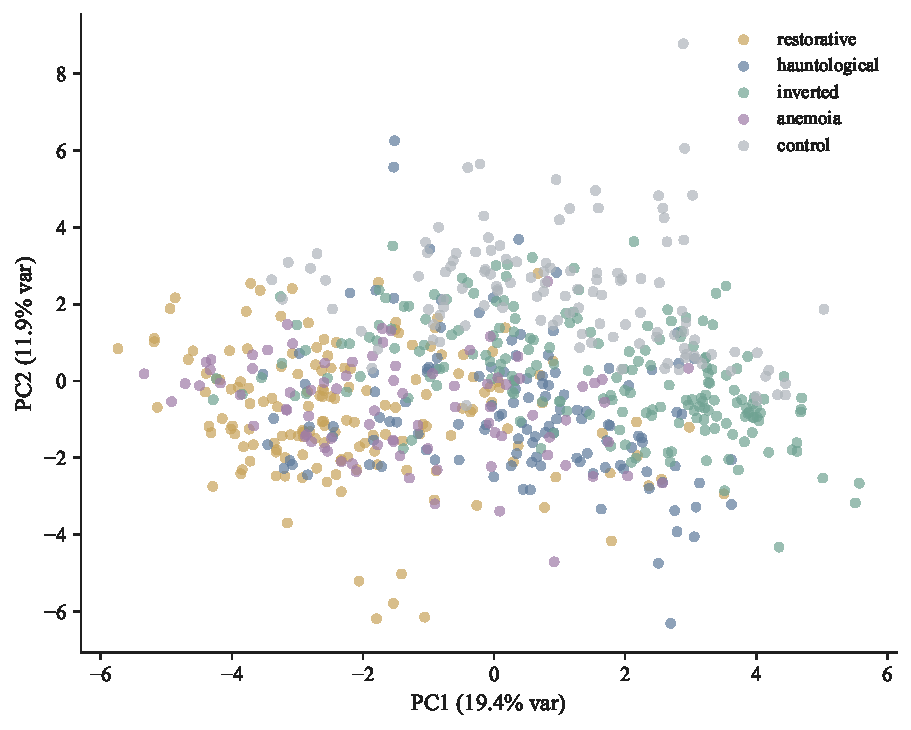
\includegraphics[width=0.72\linewidth]{figures/fig1_pca.pdf}
\caption{PCA of the standardized $681\times37$ design matrix, colored by cluster.
Restorative (gold) partially separates from the desaturated hauntological/anemoia
clusters and inverted (green, liminal) leans toward the absence-dominated region, with
heavy overlap (silhouette $\approx0$; classifiable, short of a clean partition).}
\label{fig:pca}
\end{figure}

\begin{figure}[htbp]
\centering
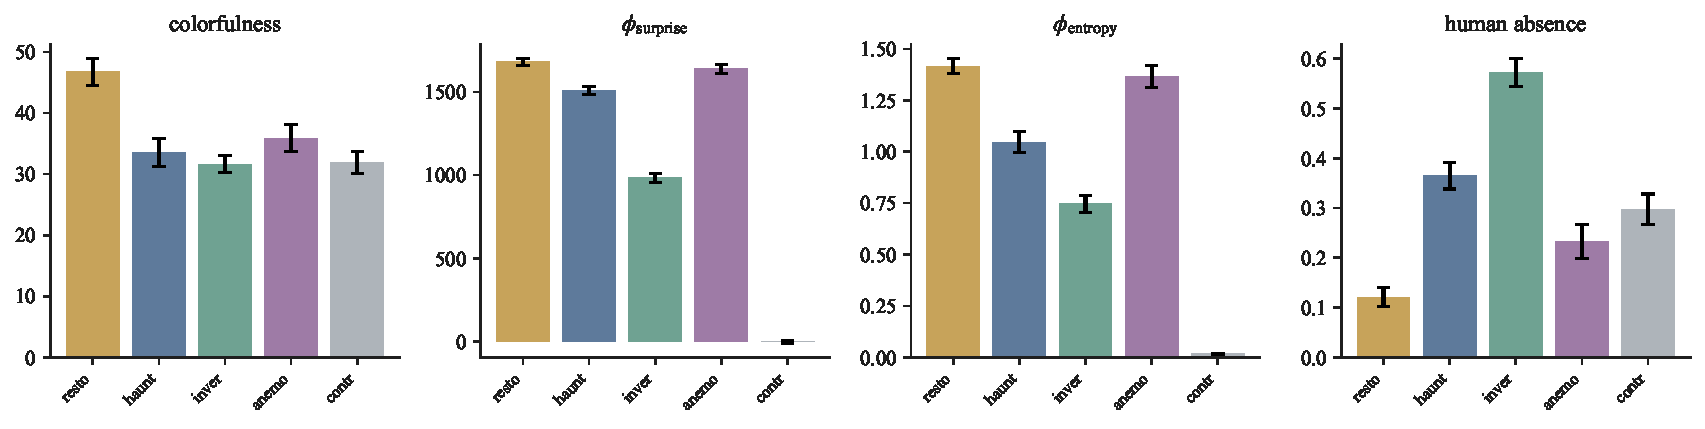
\includegraphics[width=\linewidth]{figures/fig2_eerie.pdf}
\caption{Affective spectrum by cluster (mean $\pm$ SEM): colour warmth (restorative
high), $\phi_{\text{surprise}}$ and $\phi_{\text{entropy}}$ (controls $\approx0$
by construction, see firewall discussion), and structural human absence (inverted
high). The clusters trace a warmth-to-absence gradient; cross-cluster differences are
descriptive (see text).}
\label{fig:eerie}
\end{figure}

The per-cluster means
(Table~\ref{tab:means}, Fig.~\ref{fig:eerie}) trace a descriptive warmth-to-absence gradient: colour warmth is highest
in restorative (colourfulness 46.7 vs.\ $\sim$32-36 elsewhere) and structural
\textsc{human\_absence} runs the opposite way, peaking in inverted (0.57). We flag this
as descriptive and partly confounded: colourfulness is precisely a dimension the
aesthetics manipulate in post-processing and our encyclopedic corpus lacks, so the
restorative warmth here is as much ``photos of nature'' as ``Frutiger Aero'' (see
Limitations).

The scene-matched, stratified contrast that controls
for subject matter holds scene category fixed and varies only population. Of the 194
inverted images, $170$ carry one of seven shared scene categories; the remaining $24$ are
generically tagged (waiting room, hotel corridor, analog-horror frames) with no populated
control counterpart and are excluded from this analysis. The matched cells appear in
Table~\ref{tab:scenematch}. Pooled across categories the effect is large
(\textsc{human\_absence} $d=0.75$). That pooled estimate is inflated by differing category
composition; the within-category effect is a sample-weighted $d=0.38$ (95\%
CI $[0.14,0.68]$) for \textsc{human\_absence} and $0.29$ ($[0.03,0.59]$) for
\textsc{emptiness}: modest,
positive, and reliably above zero, with the effect corridor-weighted (corridor is $77/170$ of the
tagged inverted images, and its own cell $d=0.35$ has a CI spanning zero).

The structure across cells is the most interesting result. The effect is strong
precisely where emptiness violates an occupancy expectation (classroom $0.76$, office
$0.67$, swimming pool $0.56$) and vanishes where ``empty'' is the ordinary state of
the scene (parking lot $0.04$, playground $-0.06$). Individual cells are noisy (small
$n$; CIs in Table~\ref{tab:scenematch}), so this gradient is preliminary, and it is
exactly what Fisher's eerie predicts at the scene level: the
unease tracks expected presence above emptiness per se. It yields the paper's sharpest
pre-registerable hypothesis: human unease ratings should follow the same ordering,
highest for empty-when-usually-occupied scenes (\S Discussion).

\begin{table}[htbp]
\centering
\caption{Scene-matched inverted-vs-control cells, within-category Cohen's $d$ for
\textsc{human\_absence} with bootstrap 95\% CIs ($d$ for \textsc{emptiness} shown for
reference). The effect is large where emptiness violates occupancy expectation and absent
where empty is ordinary; small cells are individually unstable. Pooled $d=0.75$ is
composition-inflated.}
\label{tab:scenematch}
\small
\begin{tabular}{lrrlr}
\toprule
scene & inv.\ $n$ & ctl.\ $n$ & $d$ human\_abs.\ [95\% CI] & $d$ empt. \\
\midrule
classroom     & 12 & 18 & $\phantom{-}0.76$ \,[0.08, 1.80]\,$^\dagger$ & 0.36 \\
office        & 11 & 27 & $\phantom{-}0.67$ \,[0.06, 1.57]\,$^\dagger$ & 0.33 \\
swimming pool & 19 & 7  & $\phantom{-}0.56$ \,[0.01, 1.07]\,$^\dagger$ & 0.52 \\
shopping mall & 24 & 19 & $\phantom{-}0.37$ \,[$-0.23$, 1.01] & 0.00 \\
corridor      & 77 & 18 & $\phantom{-}0.35$ \,[$-0.12$, 0.94] & 0.41 \\
parking lot   & 19 & 15 & $\phantom{-}0.04$ \,[$-0.62$, 0.67] & 0.17 \\
playground    & 8  & 16 & $-0.06$ \,[$-0.86$, 0.84]\,$^\dagger$ & 0.13 \\
\midrule
\multicolumn{3}{l}{weighted within-category} & $\phantom{-}0.38$ \,[0.14, 0.68] & 0.29\,[0.03, 0.59] \\
\bottomrule
\end{tabular}\\[2pt]
{\footnotesize $^\dagger$ small cell ($\min n<15$); per-cell $d$ unstable, interpret via CI.}
\end{table}

In embedding space the inverted/control gap is larger, with a caveat:
$\phi_{\text{typ}}$ is also a distance-from-control measure (squared Mahalanobis to the
per-scene control centroid), so it shares the domain-shift concern of
limitation~(iii), only partly mitigated by being computed within scene. Reported as a
percentile to avoid the dimensionality-inflated raw values ($-1480$ vs.\ $-41$): control
median $38$ (90th percentile $64$) vs.\ inverted median $1387$.

The firewall bounds what this can show: controls score
$\phi_{\text{surp}}\approx0$ and entropy $0.02$ by construction (the PCA basis and scene
classifier are fit on controls). The corollary, stated plainly: ``all aesthetic clusters
are off-manifold'' is partly tautological: any image distributionally unlike the controls
reads as deviant, and $\phi_{\text{surp}}$ conflates affective deviance with mundane
distributional shift. Because every image (controls included) comes from one source
(Wikimedia), photographer/scan-artifact shift is reduced while content shift remains; we
therefore treat $\phi_{\text{surp}}$ and $\phi_{\text{ent}}$ as hypothesis-generating
measures only.

Retro-futurism is conceptually central and empirically under-sampled: the
optimistic strand of retro-futurism (Googie, atomic-age, synthwave) collected adequately
($n=15$, folded into restorative), while the decayed/hauntological strand (cassette
futurism, dieselpunk) is almost absent from open-license banks ($n=1$). We therefore
do not report the within-domain restorative-vs-hauntological retro-futurism
contrast here: the corpus cannot yet support it. The same-subject, opposite-affect comparison
would make a clean future test, and a targeted, properly licensed collection is a priority for
follow-up work.

The two measures of the eerie dissociate: segmentation
\textsc{human\_absence} separates inverted from control (0.57 vs.\ 0.30), while the
object-level \textsc{exp\_absent} stays flat (0.74 vs.\ 0.78), since openly licensed ``populated''
scenes are often architectural photographs with few people, so the detector finds little
to violate. Structural/configural absence is the cleaner measure of the eerie in this
corpus.

\begin{figure}[htbp]
\centering
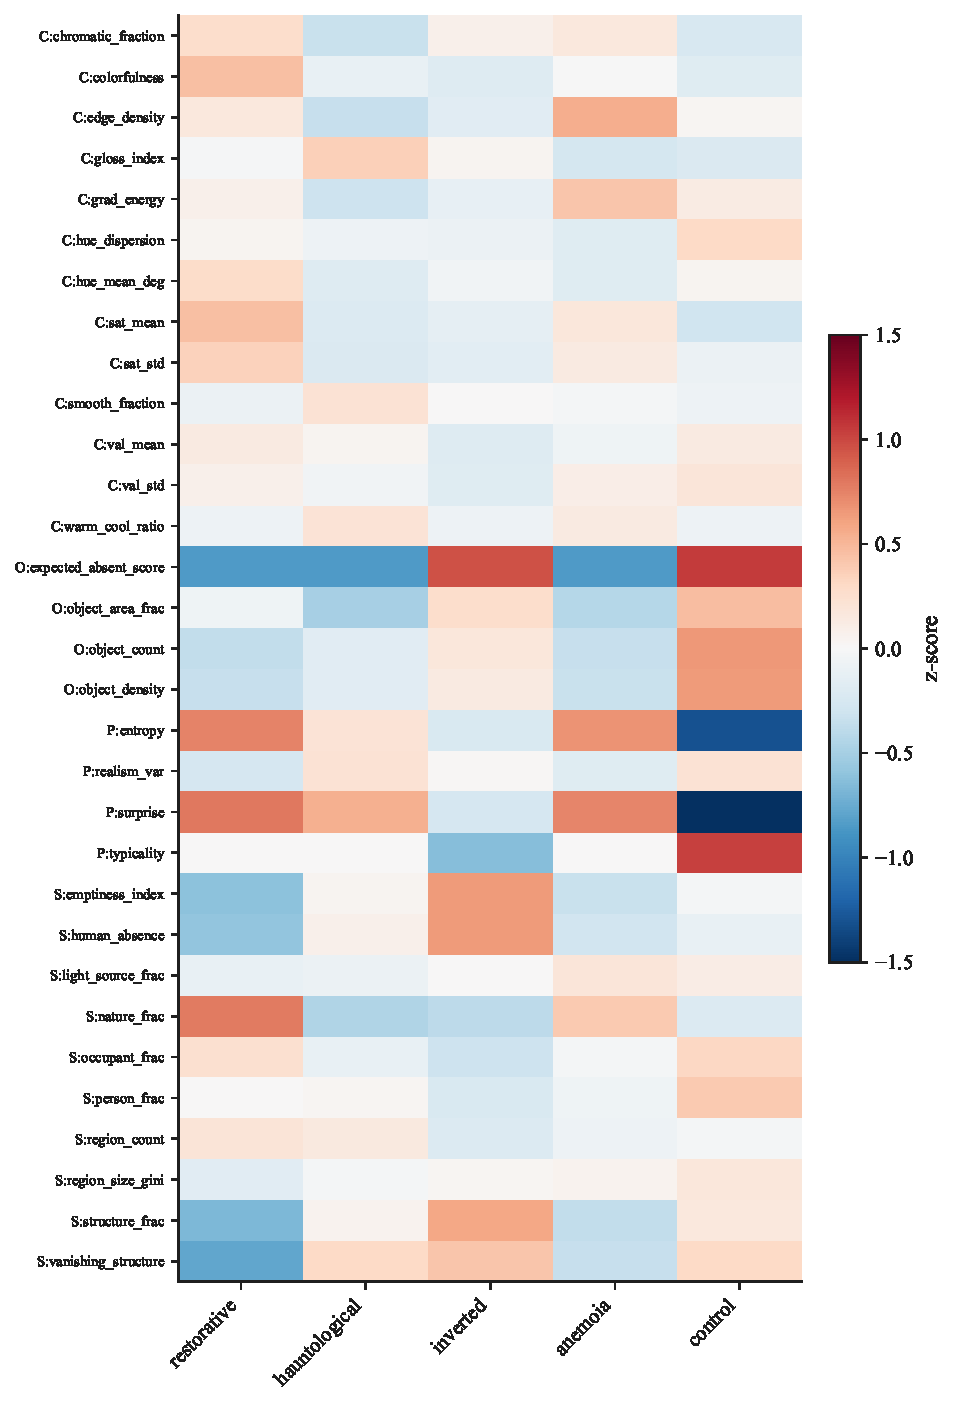
\includegraphics[width=0.62\linewidth]{figures/fig3_heatmap.pdf}
\caption{Standardized ($z$-scored) feature means by cluster across all 31 numeric
features (C: colour, S: segmentation, O: object, P: $\phi$). Restorative is marked by
colour warmth, inverted by structural absence and strongly negative typicality.}
\label{fig:heatmap}
\end{figure}


To test whether the affective structure is an artifact of our hand-built features or a
property of the stimuli recoverable by an independent mechanism, we probed every image with
CLIP \citep{radford2021} as a zero-shot observer: for each of four theory-relevant
axes (eerie, nostalgic, abandoned, dreamlike) we computed $P(\text{positive pole})$ over
prompt-ensembled contrastive text probes. CLIP is trained on web-scale human image-text
pairs, so its alignments encode aggregated human associations, a semantics-based signal
computed along an entirely different path from the perceptual axes and $\phi$ coordinates.
It stands in for human affect at one remove.

The main contrast replicates: CLIP rates the inverted cluster most eerie ($0.67$) and
restorative least ($0.44$), with an inverted-vs-control eerie difference of $d=0.72$ (95\%
CI $[0.47,0.99]$), comparable to or larger than the structural metric, by a different
measurement mechanism. CLIP nostalgia peaks for the hauntological cluster (vaporwave), as
expected, and the four zero-shot affect axes alone classify the five clusters at
$0.45$ (chance $0.20$). Two independent methods thus recover the same cluster ordering.

The two methods are complementary, and they disagree where it matters. At the image level
CLIP eeriness correlates only modestly with structural \textsc{human\_absence}
($r=0.29$): the methods triangulate one construct while measuring distinct features.
And CLIP eeriness does not reproduce the scene-level occupancy gradient: the
within-scene inverted-vs-control effect is present, with its ordering across scenes differing
(e.g.\ corridor near-zero, playground large), opposite the structural pattern. Structural
absence and semantic eeriness agree that the inverted pole is eerie and differ on
where, indicating that the occupancy moderator is method-dependent. Two independent
measurements thus converge on the same inverted-vs-rest contrast.

\section{Frontier-panel confusion matrix}

Figure~\ref{fig:confusionheat} gives the full three-model confusion behind the flow in
Fig.~\ref{fig:vlmbreak}: human-assigned mode against VLM consensus mode, row-normalised, with the
per-mode mode-match recall.

\begin{figure}[htbp]
\centering
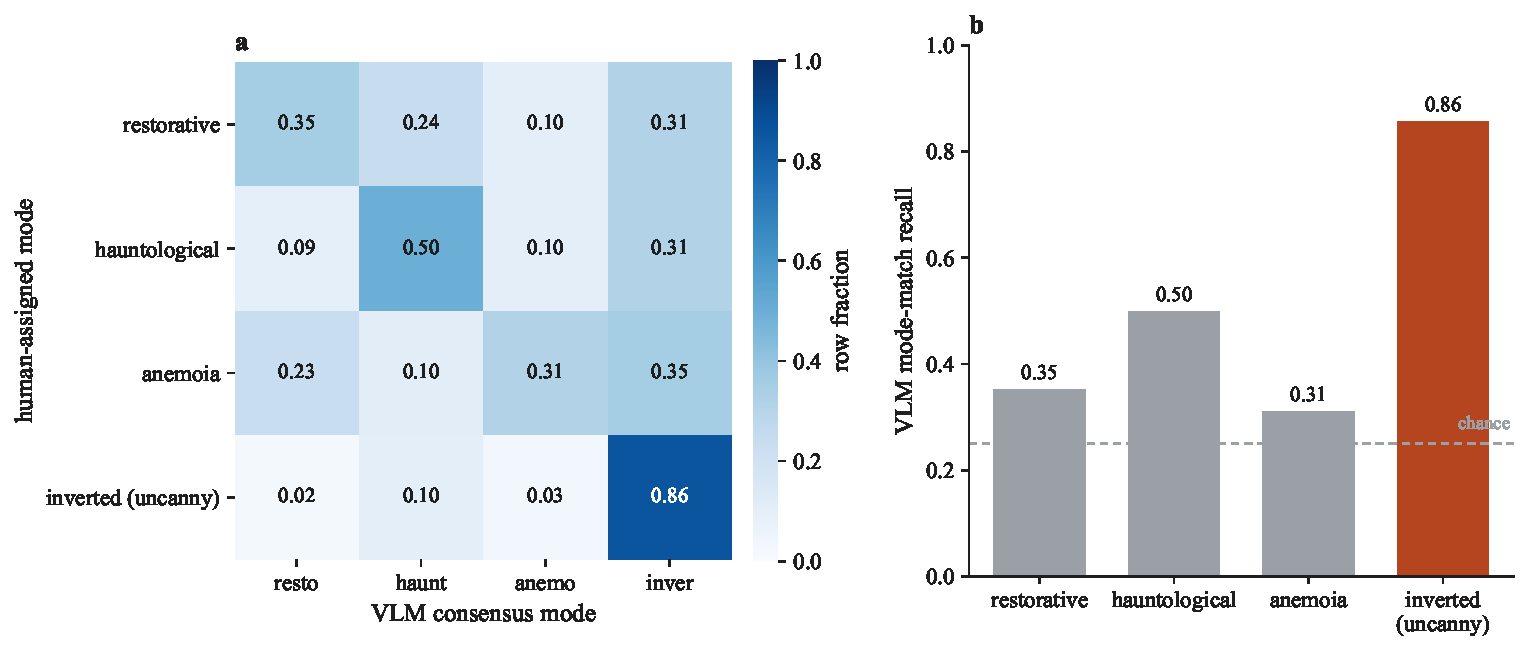
\includegraphics[width=\linewidth]{figures/vlm_where_it_breaks.pdf}
\caption{Three-model VLM confusion on the are.na images. (a) Human-assigned mode (rows) vs.\ VLM
consensus mode (columns), row-normalised; every non-uncanny class leaks into the ``inverted''
column. (b) Per-mode mode-match recall. This is the matrix that Fig.~\ref{fig:vlmbreak} summarises
as a flow.}
\label{fig:confusionheat}
\end{figure}

\end{document}